\chapter{Diseño e Implementación}
\label{cap:capitulo4}


\vspace{1cm}
El principal objetivo de este TFG es desarrollar un sistema autónomo de navegación sigue-carril para un dron basado en aprendizaje por refuerzo, siendo este capaz de desenvolverse
por carreteras urbanas con un comportamiento reactivo.
En este capítulo se desarrolla como se ha alcanzando este objetivo. En primer lugar se diseña la infraestructura de comunicaciones entre el entorno de simulación y las diversas 
plataformas de desarrollo. Esta 
infraestructura de comunicaciones, permite la transferencia de datos en tiempo real y la integración de diferentes módulos del sistema, garantizando 
una comunicación fluida y eficiente.
A continuación, se desarrolla el sistema perceptivo mediante el uso de inteligencia artificial junto con la implementación de comportamientos autónomos tradicionales empleados
 en diferentes robots, como el seguimiento de carriles. Entre los métodos utilizados se incluye 
el control clásico basado en controladores y métodos de control avanzados basados en aprendizaje por refuerzo, con el objetivo de que el dron aprenda y se 
adapte a distintos escenarios urbanos. 
Una vez desarrollados estos comportamientos, se procede a realizar una evaluación de los comportamientos obtenidos. Se recopilan
diversas métricas para determinar la efectividad de cada enfoque y adaptabilidad del dron. 
Finalmente, se analizan los resultados y se realiza una comparativa, destacando las ventajas y limitaciones de cada enfoque, 
proporcionando así una visión global del desempeño del sistema autónomo 
de navegación del dron en carreteras.

\section{Arquitectura}
\label{sec:Arquitectura}

La arquitectura propuesta para este trabajo se muestra en la figura \ref{fig:infraestructura}. Consta de dos componentes principales 
comunicados entre sí por medio de un router y conexión Ethernet: el entorno de simulación  y las plataformas de desarrollo. Estos componentes 
están separados en dos ordenadores distintos, siendo PC1 el entorno de simulación y PC2 las plataformas de desarrollo junto con los algoritmos de percepción y de sigue-carril. 
El objetivo de esta separación en dos ordenadores diferentes es para poder dividir la carga computacional, ya que una sola máquina es incapaz de ejecutar el simulador y los algoritmos 
desarrollados en este TFG dada la alta demanda computacional del simulador Airsim. 

\begin{figure} [H]
  \begin{center}
    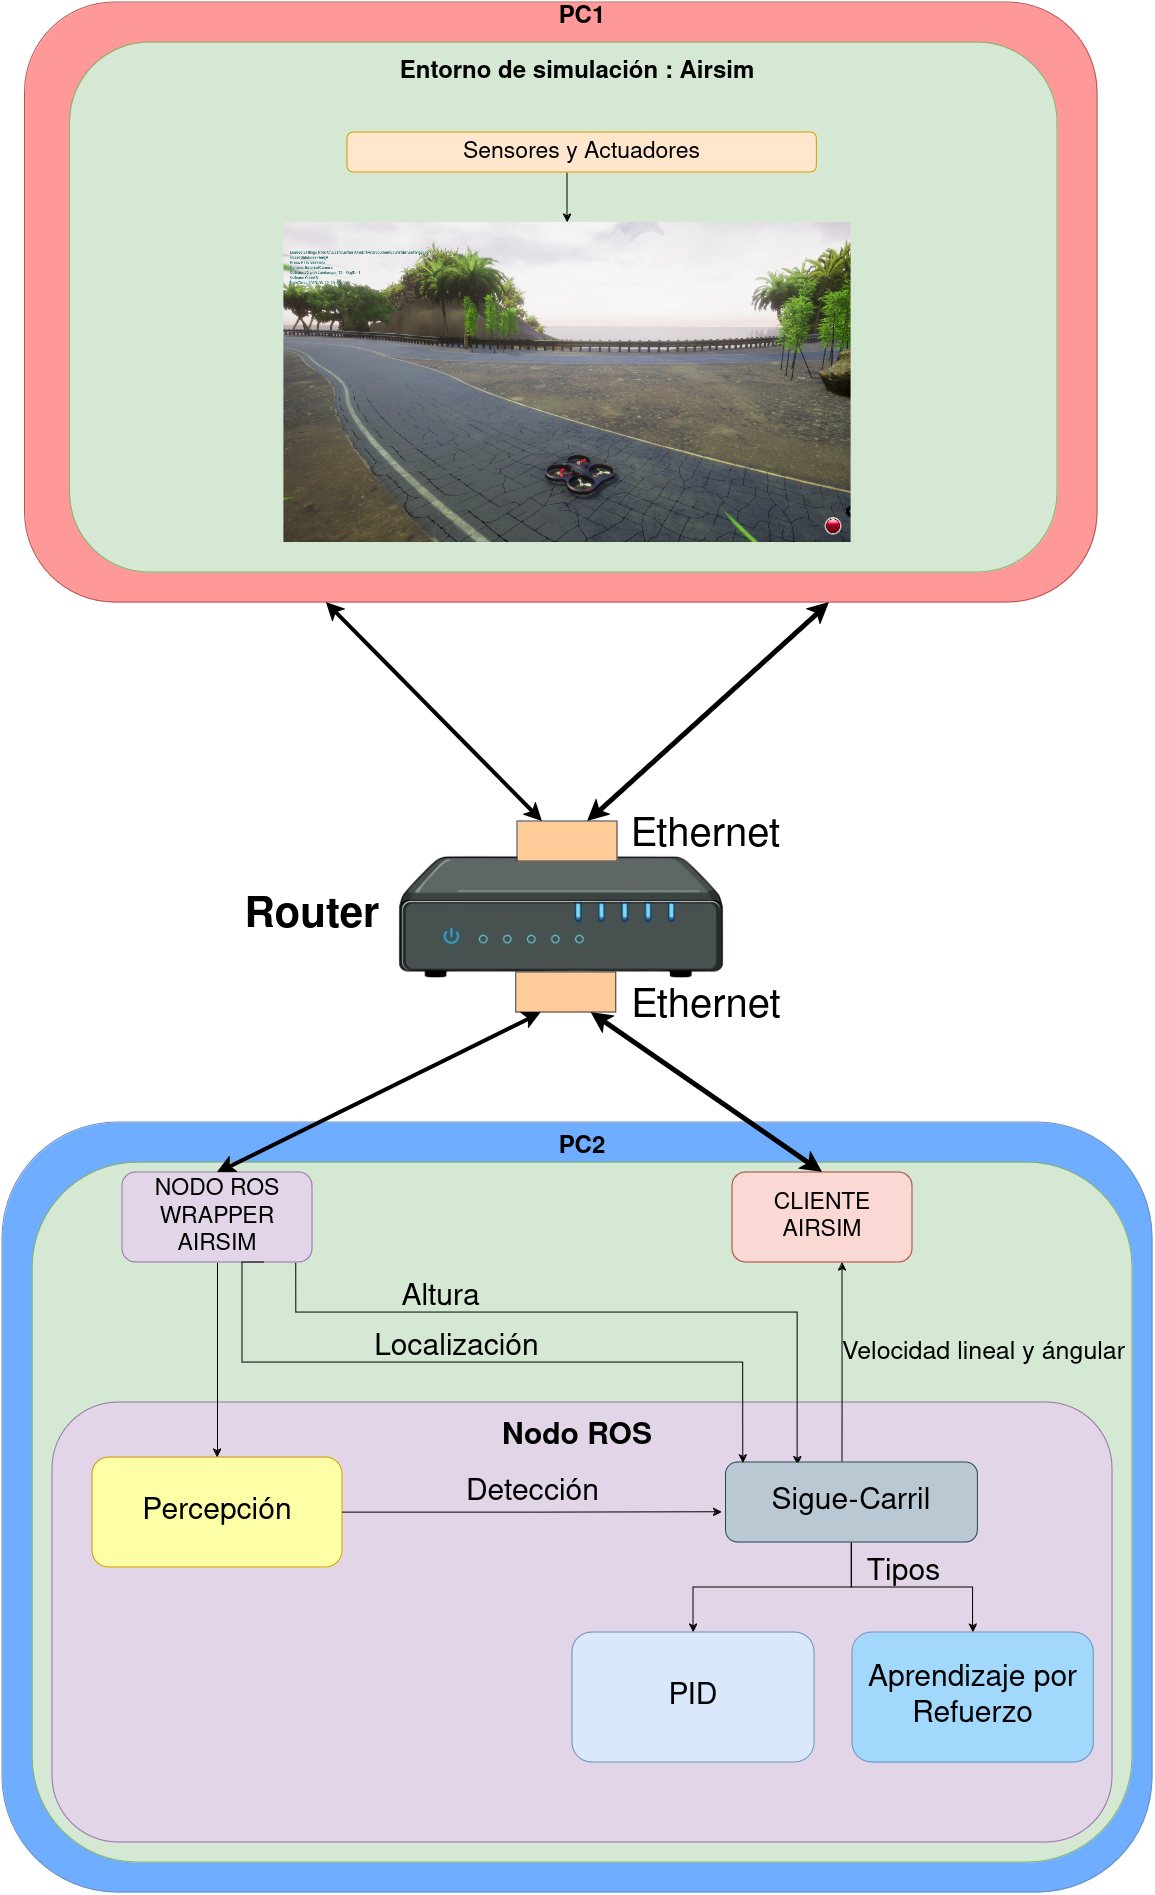
\includegraphics[scale=0.30]{figs/Diseño/Comunicaciones/diagrama_arquitectura_2.png}
  \end{center}
  \caption{Arquitectura general del desarrollo en este TFG}
  \label{fig:infraestructura}
  \vspace{-1.5em}
\end{figure}

Por un lado, el primer componente está compuesto por el entorno de simulación Airsim, ejecutado en el PC1. Incluye la configuración de sensores y actuadores necesarios 
para la navegación del dron. La comunicación entre este componente y el segundo componente (PC2), se realiza a través de dos interfaces principales: 

\begin{enumerate}
  \item \textbf{ROS Wrapper Airsim Node}: Este componente actúa como una interfaz que facilita la integración de Airsim con el middleware ROS. A través del ROS Wrapper Airsim, 
  se recogen tres tipos de salidas: 
    \begin{enumerate}
      \item \textbf{Imágenes RGB}: Capturadas por las cámaras a bordo del dron, estas imágenes son fundamentales para el sistema perceptivo, permitiendo la detección y el 
      seguimiento del carril.
      \item \textbf{Altura}: Obtenida a través del sensor Lidar, esta medida es esencial para conocer la altura a la que vuela el dron durante su navegación. 
      \item \textbf{Localización}: Proporcionada por el GPS, esta información permite conocer la posición del dron en el entorno simulado. 
    \end{enumerate}

  \item \textbf{Client Airsim}: Este componente permite el control del dron, gestionando las velocidades lineales y angulares necesarias para su navegación. 
\end{enumerate}

Dentro de PC2, se encuentra el componente que encapsula el sistema perceptivo y el seguimiento de carril, actuando como el núcleo de 
procesamiento. Este componente recibe y procesa las entradas de los sensores (imágenes RGB, altura y localización), y genera velocidades lineales y angulares.

Toda la funcionalidad se implementa dentro de dos submódulos:
\begin{enumerate}
  \item \textbf{Percepción}: Utilizando las imágenes RGB proporcionadas por ROS Wrapper Airsim, este sistema procesa la información
  visual para detectar el carril en el que debe navegar el dron. La detección del carril es fundamental para la ejecución del comportamiento sigue-carril, que guía al dron 
  a lo largo del carril deseado. 
  \item \textbf{Sigue-Carril}: Este comportamiento se encarga de seguir el carril en función de la información obtenida de la percepción. Dentro de este componente, se 
  utiliza dos enfoques diferentes: 
  \begin{enumerate}
    \item \textbf{PID}: Un enfoque clásico de control que ajusta las velocidad angulares en función de las desviaciones del carril detectado. En este controlador, la velocidad lineal 
    del dron es constante.
    \item \textbf{Aprendizaje por Refuerzo}: Un enfoque más avanzado que utiliza técnicas de aprendizaje automático para optimizar el comportamiento del dron. Este método 
    permite al dron aprender de su entorno en diferentes condiciones, dotandole de la capacidad de generalizar el comportamiento aprendido, provocando que sea capaz de funcionar correctamente
    en entornos nunca vistos anteriormente.

  \end{enumerate}

  Ambos enfoques de control generan comandos de velocidades lineales y angulares que son enviados al Client Airsim. Este, a su vez, traduce estos comandos en acciones físicas 
  en el entorno simulado, permitiendo un movimiento controlado y preciso del dron. 


\end{enumerate}

\section{Configuración del sistema distribuido}
\label{distribución}
En el desarrollo de este TFG, se ha decidido adoptar un enfoque distribuido. El entorno de simulación, compuesto por Airsim y UnrealEngine, se ejecuta en un ordenador de sobremesa con un sistema 
operativo Windows 10 y una GPU Nvidia RTX 2070 Super. Por otra parte, las plataformas de desarrollo y control, que incluyen ROS, AirSim ROS Wrapper Node y Client Airsim se ejecutan en un ordenador
portátil con un sistema operativo Ubuntu 20.04 y una GPU Nvidia RTX 2070.
Esta propuesta se tomó con la iniciativa de no encapsular en un único componente el entorno de simulación y las plataformas de desarrollo. Inicialmente, todo el sistema 
seguía una configuración centralizada en un solo equipo con Ubuntu 20.04, generando cuellos de botella y limitando al rendimiento del sistema. Para solventar estos problemas, 
se configuró una infraestructura distribuida entre dos ordenadores distintos, dividendo así la carga de trabajo entre los dos sistemas.

Al principio del desarrollo, en esta distribución de equipos, se utilizó una comunicación con PX4 y Mavros, siguiendo la documentación oficial\footnote{\url{https://docs.px4.io/main/en/simulation/}} 
junto con el entorno de simulación Airsim. Sin embargo, se decidió cambiar por una nueva configuración que emplea ROS Wrapper Airsim Node y Client Airsim, ya que 
la comunicación original añadía una capa de procesamiento adicional, produciendo bajos rendimientos que afectaba a la sincronización con el simulador. 

En resumen, el sistema de comunicaciones se compone de dos ordenadores interconectados en la misma red. El diagrama 
de comunicaciones ilustrado en la figura \ref{fig:diagramadeAirsim}, muestra esta implementación distribuida en diferentes ordenadores. Cada ordenador asume roles distintos: 
El primer ordenador ejecuta el entorno de simulación en cambio el segundo ordenador, gestiona las plataformas de desarrollo en donde se implementan los algoritmos 
de percepción y seguimiento de carril. Ambos ordenadores se comunican a través de un router teniendo cada uno una dirección IP distinta. 

\begin{figure} [H]
  \begin{center}
    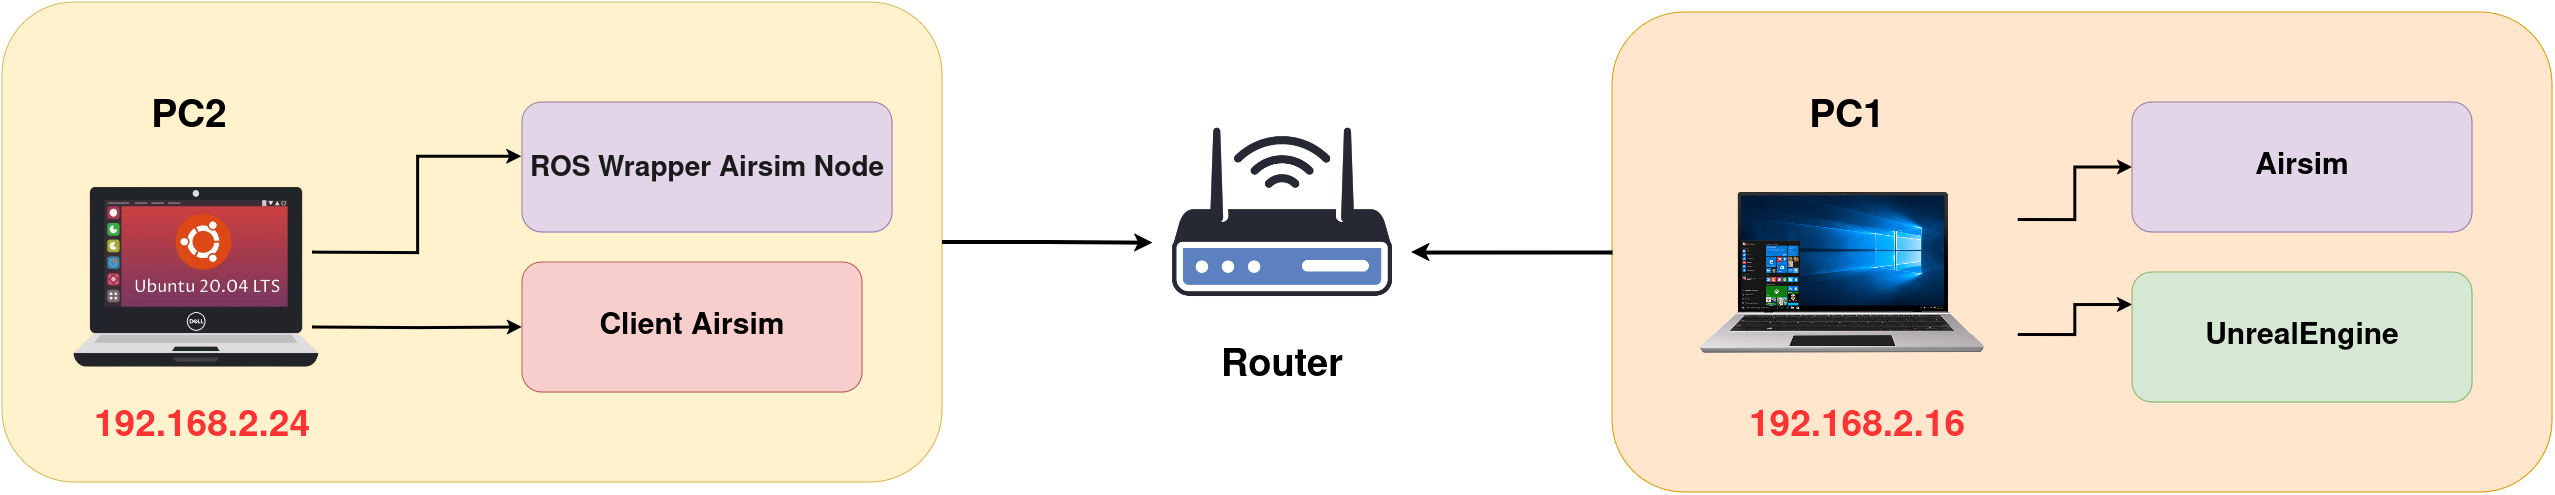
\includegraphics[scale=0.18]{figs/Diseño/Comunicaciones/comunicaciones.png}
  \end{center}
  \caption{Diagrama de comunicaciones}
  \label{fig:diagramadeAirsim}
\end{figure}

\subsection{Preparación del entorno de simulación}
\label{sec:Preparación_entorno}

Como se menciona en la sección \ref{sec:Airsim}, se utiliza como simulador Airsim junto con el motor UnrealEngine. Para construir el entorno de simulación, primero
se necesita instalar UnrealEngine. Para ello, se sigue las instrucciones marcadas por la página oficial de Epic Games\footnote{\url{https://www.unrealengine.com/en-US/download}}, 
utilizando la versión 4.27.2.

Una vez que UnrealEngine esté instalado, se procede a configurar el entorno de simulación mediante el archivo settings.json. Por defecto, al ejecutar Airsim 
por primera vez, el simulador crea este archivo automáticamente dentro de una carpeta denominada Airsim en la carpeta Documentos en Windows. 


\subsubsection{Configuración del dron y del entorno}
\label{subsec:Configuración del dron y del entorno}
En primer lugar se utiliza el mapa de simulación Coastline de entre los diferentes mapas que te ofrece Airsim para Windows. Al descargar esta carpeta, 
se obtiene un fichero ejecutable para abrir el entorno con Airsim, junto con carpetas de modelos de simulación como las carreteras, montañas y vegetación. Dentro de estas carpetas, se eliminan dichos componentes 
de simulación que pueden dificultar al sistema perceptivo, como plantas y señales de tráfico que se ubican en las carreteras, facilitando así la percepción del entorno 
y haciéndolo más manejable. En la figura \ref{fig:CoastlineModificado} se muestra marcado en color rojo, los componentes eliminados del entorno para facilitar al sistema 
perceptivo.

\begin{figure} [H]
  \begin{center}
    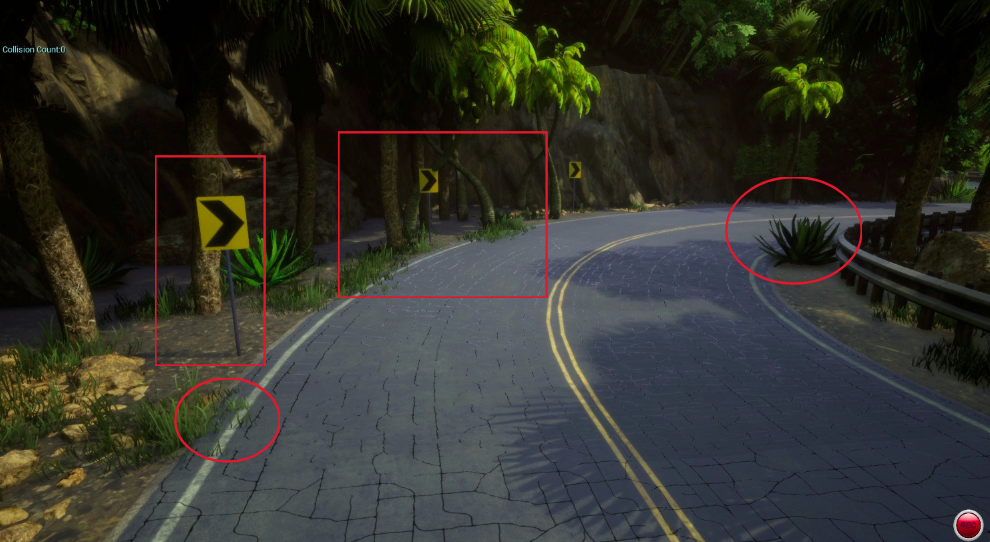
\includegraphics[scale=0.3]{figs/Diseño/coastline3.png}
  \end{center}
  \caption{Visualización del entorno original ilustrando los objetos que dificultan al sistema perceptivo}
  \label{fig:CoastlineModificado}
  \vspace{-1.5em}
\end{figure}
Cuando el fichero settings.json este creado, ya se puede equipar al dron con características como qué sensores va a utilizar, 
el tipo de vehículo, el tipo de simulación, la comunicación y más. Como se muestra en la figura \ref{cod:settings}, se definen como sensores el Lidar para saber a que altura
esta volando el dron respecto al suelo, el GPS para conocer la localización que tiene el dron en el entorno y la cámara con imágenes
RGB. Cada sensor debe llevar su propia configuración, siguiendo los parámetros que dicta la guía oficial de Airsim\footnote{\url{https://microsoft.github.io/AirSim/sensors/}}
. La cámara tiene una peculiaridad de que se configura siendo otro sensor a parte de la lista de sensores de Airsim, consta de varios parámetros que se tienen que configurar como 
el tamaño de la imagen, el uso de ROS, los FPS de la imagen transmitida, la posición, etc. 
Respecto de los actuadores, no se debe realizar ninguna configuración especial para ellos.

\begin{figure}[H]
  \centering
  \begin{multicols}{2}
    \begin{lstlisting}[language=json,basicstyle=\tiny,numbers=none]
{
  "SettingsVersion":1.2,
  "SimMode":"Multirotor",
  "ClockType":"SteppableClock",
  "Vehicles":{
     "Drone":{
        "VehicleType":"SimpleFlight",
        "ControlIp":"remote",
        "LocalHostIp":"192.168.2.16",
        "Sensors":{
           "LidarCustom":{
              "SensorType":6,
              "Enabled":true,
              "Range":10,
              "NumberOfChannels":16,
              "RotationsPerSecond":10,
              "PointsPerSecond":10000,
              "X":0,
              "Y":0,
              "Z":-1,
              "DrawDebugPoints":false,
              "DataFrame":"SensorLocalFrame"
           },
           "Gps":{
              "SensorType":3,
              "Enabled":true,
              "EphTimeConstant":0.9,
              "EpvTimeConstant":0.9,
              "EphInitial":25,
              "EpvInitial":25,
              "EphFinal":0.1,
              "EpvFinal":0.1,
              "EphMin3d":3,
              "EphMin2d":4,
              "UpdateLatency":0.2,
              "UpdateFrequency":50,
              "StartupDelay":1
           }
        }
     }
  }
}
    \end{lstlisting}
    \columnbreak
    \begin{lstlisting}[language=json,basicstyle=\tiny,numbers=none]
{
   "Cameras":{
     "front_center_custom":{
        "CaptureSettings":[
           {
              "PublishToRos":1,
              "ImageType":0,
              "Width":620,
              "Height":620,
              "FOV_Degrees":90,
              "ImageRate_FPS":30,
              "TargetGamma":1.5,
              "AutoExposure":true,
              "MotionBlur":false,
              "PostProcess":true
           }
        ],
        "X":0.50,
        "Y":0,
        "Z":0.10,
        "Pitch":0,
        "Roll":0,
        "Yaw": 0
     }
   },
   "X": 22.474933624267578,
   "Y": -25.63629913330078,
   "Z":  0,
   "Pitch": 0,
   "Roll": 0,
   "Yaw":  30
}
    \end{lstlisting}
  \end{multicols}
  \caption[Configuración del dron mediante el fichero settings.json]{Configuración del dron mediante el fichero settings.json}
  \label{cod:settings}
  \vspace{-1.5em}
\end{figure}

Si no se define la posición inicial del dron como aparece en la última parte del fichero settings.json, por defecto el propio simulador te establece el dron en el punto que decida Airsim.

Para poder utilizar Airsim ROS Wrapper y Client Airsim junto con el simulador, se debe especificar la dirección IP en donde se encuentra el simulador Airsim. En el código 
\ref{cod:roslaunch} se muestra la ejecución del launcher \texttt{airsim\_node.launch} proporcionado por Airsim ROS Wrapper y en el código \ref{cod:airsim} se muestra el uso del método
\texttt{airsim.MultirotorClient}
para establecer la comunicación con Airsim.

\begin{code}  [H]
  \begin{lstlisting}
    roslaunch airsim_ros_pkgs airsim_node.launch output:=screen host:=192.168.2.16
  \end{lstlisting}
  \caption[comando]{Lanzamiento del nodo AirSim ROS Wrapper Node especificando la dirección IP del simulador}
  \label{cod:roslaunch}
\end{code} 

\begin{code}  [H]
  \begin{lstlisting}[language=Python]
    import airsim
    client_airsim = airsim.MultirotorClient(ip="192.168.2.16")
  \end{lstlisting}
  \caption[comando]{Conexión al simulador Airsim utilizando Client Airsim especificando la dirección IP}
  \label{cod:airsim}
\end{code} 



\section{Comportamiento de seguimiento de carril con drones}
\label{sec:Comportamiento de seguimiento de carril con drones}
Para desarrollar el comportamiento de seguimiento de carriles, es crucial diseñar un sistema perceptivo que detecte el carril a seguir. Una vez 
construido este sistema, se procede al desarrollo de un algoritmo de seguimiento de carril. Dicho algoritmo se enfoca en dos estrategias distintas 
para comandar las velocidades lineales y angulares del dron, como se comenta en la sección \ref{sec:Control}. 
\subsection{Percepción}
\label{sec:Percepción}
En las fases iniciales del desarrollo del sistema perceptivo, se optó por emplear técnicas de visión tradicional utilizando métodos que ofrece la biblioteca 
OpenCV, tales como GaussianBlur, Canny e HoughLines. Antes de poder utilizarlos, se necesita obtener la imagen proporcionada por la cámara a bordo del dron. Esto se logra
suscribiéndose al topic \texttt{/airsim\_node/Drone/front\_center\_custom/Scene}, facilitada por el nodo AirSim ROS Wrapper Node. Posteriormente, mediante el uso de 
CvBridge\footnote{\url{http://wiki.ros.org/cv_bridge}}, se transforma la imagen al formato de OpenCV para su posterior procesamiento con esta biblioteca.

Para los métodos GaussianBlur, Canny e HoughLines se necesita trabajar con imágenes en escala de grises, por lo tanto, primero se realiza una transformación de la imagen 
de color a escala de grises. A continuación se utiliza el método GaussianBlur\footnote{\url{https://docs.opencv.org/4.x/d4/d13/tutorial_py_filtering.html}}, que aplica un desenfoque 
gaussiano a la imagen. Este proceso suaviza la imagen, reduciendo el ruido y mejorando la detección de bordes y líneas. Seguidamente, se aplica el método Canny\footnote{\url{https://docs.opencv.org/4.x/da/d22/tutorial_py_canny.html}} 
para la detección de bordes en la imagen. Finalmente, se aplica el método HoughLines\footnote{\url{https://docs.opencv.org/3.4/d9/db0/tutorial_hough_lines.html}} 
para detectar líneas en la imagen mediante la transformación de Hough, permitiendo identificar líneas rectas dentro de una imagen. 

El resultado final de la aplicación de estos algoritmos de visión clásica se puede observar en la figura \ref{Vision_clasica}. En la parte superior de la figura se presentan diferentes segmentos
de carril: Una zona curvada, una zona recta y una zona semirrecta. Estas imágenes representan la entrada original capturada por la cámara del dron. En la parte inferior de la figura, 
se muestran los resultados de la detección de líneas sobre las imágenes originales mediante el uso de los algoritmos mencionados. En la zona recta se puede ver como las líneas
detectadas son claramente visibles y paralelas, lo que indica una correcta detección en este tipo de trayectos rectos. Mientras que en las zona curvada y la zona semirrecta, presentan
dificultades en la detección de las lineas, debido a que HoughLines esta optimizada para la detección de líneas rectas y no para la detección de líneas curvadas. 

\begin{figure}[H]
  \centering
  \begin{minipage}[t]{0.3\textwidth}
      \centering
      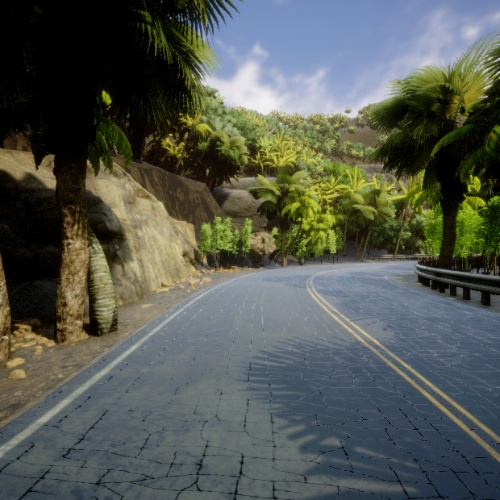
\includegraphics[width=\textwidth]{figs/Diseño/Percepcion/vision_clasica/imagen-original.jpg}
      \caption*{a: Zona curvada}
  \end{minipage}
  \hfill
  \begin{minipage}[t]{0.3\textwidth}
      \centering
      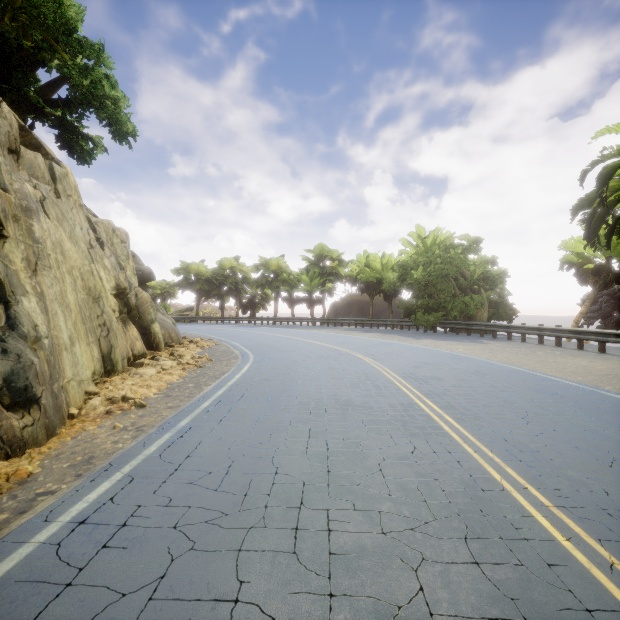
\includegraphics[width=\textwidth]{figs/Diseño/Percepcion/vision_clasica/imagen-original2.jpg}
      \caption*{b: Zona recta}
  \end{minipage}
  \hfill
  \begin{minipage}[t]{0.3\textwidth}
      \centering
      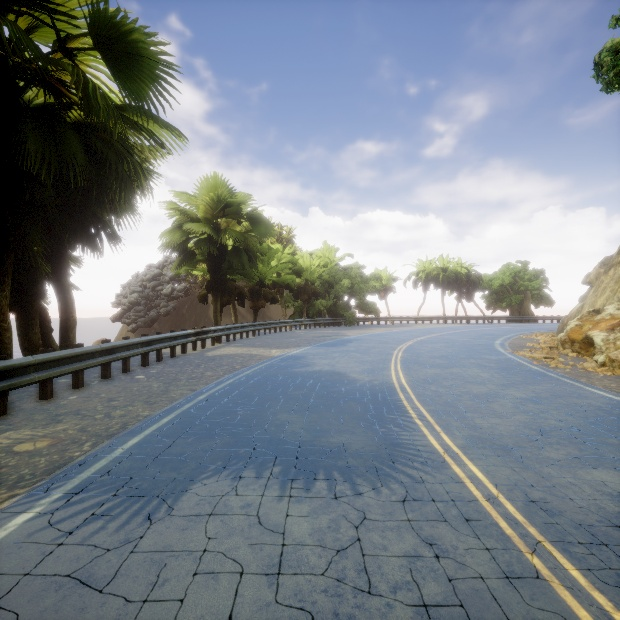
\includegraphics[width=\textwidth]{figs/Diseño/Percepcion/vision_clasica/imagen-original3.jpg}
      \caption*{c: Zona semirrecta}
  \end{minipage}
  
  \vspace{1cm}
  
  \begin{minipage}[t]{0.3\textwidth}
      \centering
      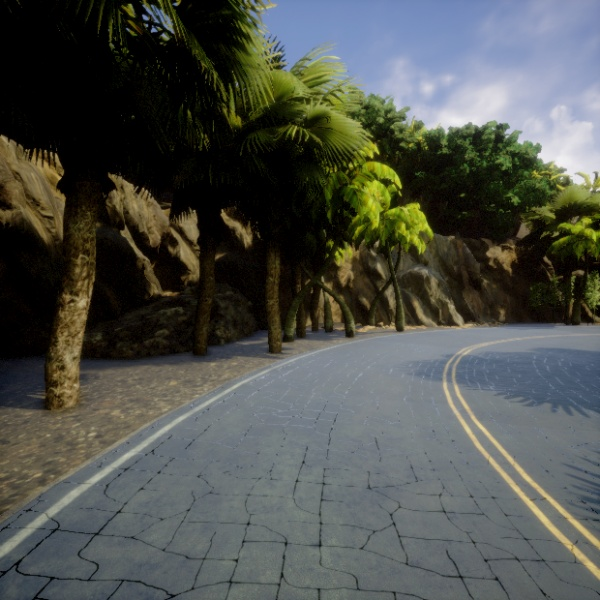
\includegraphics[width=\textwidth]{figs/Diseño/Percepcion/vision_clasica/deteccion.jpg}
      \caption*{d: Detección en la zona curvada}
  \end{minipage}
  \hfill
  \begin{minipage}[t]{0.3\textwidth}
      \centering
      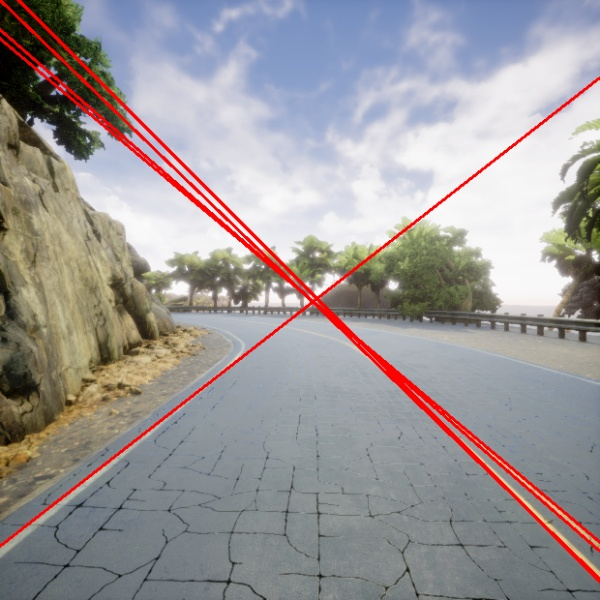
\includegraphics[width=\textwidth]{figs/Diseño/Percepcion/vision_clasica/deteccion2.jpg}
      \caption*{e: Detección en la zona recta}
  \end{minipage}
  \hfill
  \begin{minipage}[t]{0.3\textwidth}
      \centering
      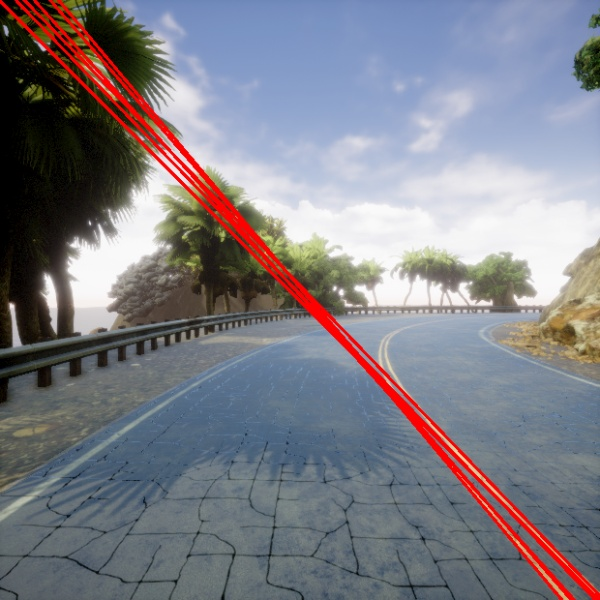
\includegraphics[width=\textwidth]{figs/Diseño/Percepcion/vision_clasica/deteccion3.jpg}
      \caption*{f: Detección en la zona semirrecta}
  \end{minipage}
  \caption{Resultado de la detección de líneas utilizando visión clásica}
  \label{Vision_clasica}
\end{figure}

Debido al mal funcionamiento de estos algoritmos de visión clásica en la detección de líneas en los carriles, 
hemos optado por utilizar técnicas de Inteligencia Artificial, en especial Deep Learning, utilizando la red neuronal YOLOP. Como se comenta en la sección \ref{sec:YOLOP}, 
YOLOP es una red neuronal que realiza una detección de objetos de tráfico, una segmentación del área transitable y una detección de carriles. Es importante 
destacar que se realiza solamente la inferencia de los distintos modelos ya entrenados con datos reales que ofrece YOLOP, sin realizar un nuevo entrenamiento. Este enfoque nos permite aprovechar 
la detección de las líneas proporcionadas por la red para mejorar la percepción del entorno del dron, proporcionando una detección más robusta y precisa a una gran variedad de configuraciones
de las carreteras urbanas dentro del entorno de Airsim. 

\subsubsection{Inferencia de YOLOP}
\label{sec:Inferencia de YOLOP}

Para realizar la detección de las líneas en la carretera, se utiliza la red neuronal YOLOP\footnote{\url{https://github.com/hustvl/YOLOP}}. En primer lugar, 
se realiza la inferencia del modelo \texttt{End-to-end.pth} y más adelante la inferencia de los modelos \texttt{Yolop-320-320.onnx}, \texttt{Yolop-640-640.onnx} e 
\texttt{Yolop-1280-1280.onnx} mediante el uso de ONNX Runtime, todos ellos entrenados con datos reales. 
El archivo End-to-end.pth es un modelo preentrenado con datos reales construido en formato Pytorch que contiene los pesos y sesgos de la red neuronal después del entrenamiento. En el contexto de 
redes neuronales, \texttt{end-to-end} significa que la red se entrena para realizar todas las etapas de un proceso completo. En el caso de YOLOP, esto significa que se ha entrenado de manera integral 
para realizar simultáneamente todas sus tareas (detección de objetos, segmentación de áreas transitables y detección de líneas). Para poder cargar este modelo, se realiza 
su carga mediante el repositorio de Github\footnote{\url{https://github.com/hustvl/YOLOP}}
especificando el modelo de la red neuronal y la opción 'pretrained' definida con valor \textit{True}, especificando que los pesos del modelo de la red se cargan del archivo 
\texttt{End-to-end.pth}.

\begin{code}[h]
  \begin{lstlisting}[language=Python]
  import torch
  model = torch.hub.load('hustvl/yolop', 'yolop', pretrained=True)

  \end{lstlisting}
  \caption[Cargar modelo YOLOP con pesos preentrenados End-to-end.pth]{Cargar modelo YOLOP con pesos preentrenados End-to-end.pth}
  \label{cod:cargar_modelo}
  \end{code}  

Una vez se tenga el modelo cargado del repositorio como se ilustra en el código \ref{cod:cargar_modelo}, se puede escoger 
si se quiere realizar la inferencia mediante el uso de la CPU o el uso de la GPU. Para una mejor comportamiento de la red neuronal, se utiliza
la GPU para realizar la inferencia asignándole el dispositivo GPU como se muestra en el código \ref{cod:codeloadYOLOP}.

  
\begin{code}[h]
    \begin{lstlisting}[language=Python]
    device = torch.device("cuda" if torch.cuda.is_available() else "cpu")
    model = model.to(device)
  
    \end{lstlisting}
    \caption[Cargar modelo YOLOP escogiendo como dispositivo la GPU]{Cargar modelo YOLOP escogiendo como dispositivo la GPU}
    \label{cod:codeloadYOLOP}
    \end{code}  

      Esta red neuronal ofrece modelos con formato ONNX: \texttt{Yolop-320-320.onnx, Yolop-640-640.onnx e Yolop-1280-1280.onnx}. Estos modelos son construidos a partir del archivo 
      \texttt{End-to-end.pth} y se convierten en modelos con formato Onnx. Cada modelo proporcionado con formato onnx tiene una resolución distinta de entrada en cuanto a las dimensiones
      de las imágenes. El archivo \texttt{Yolop-320-320.onnx} necesita una entrada con unas dimensiones de 320x320 píxeles en las imágenes, el archivo \texttt{Yolop-640-640.onnx} necesita 
      una entrada con unas dimensiones de 640x640 píxeles en las imágenes y por último el archivo \texttt{Yolop-1280-1280.onnx} se necesita unas dimensiones de imágenes de 1280x1280 píxeles. 
      En cuanto al uso de estos modelos, se debe realizar la configuración de los drivers de CUDA con la versión disponible para ONNX Runtime, 
      dichas versiones tienen que ser compatible entre sí. Para llevar a cabo este proceso, se emplea la tabla requisitos proporcionada en la página oficial de ONNX Runtime\footnote{\url{https://onnxruntime.ai/docs/execution-providers/CUDA-ExecutionProvider.html}}.

      Cuando se trabaja con ONNX Runtime, se puede especificar qué proveedores de ejecución utilizar para ejecutar la inferencia del modelo de ONNX elegido. Cada proveedor 
      contiene un conjunto de núcleos optimizados para un objetivo específico (por ejemplo, CPU, GPU, IoT), cada proveedor se especifica en una lista en orden de prioridad. Para realizar 
      inferencia de estos modelos, se escoge CUDA para ejecutar mediante la GPU. En el código \ref{yolop320} se muestra la carga del modelo \texttt{Yolop-320-320.onnx} junto con la configuración
      del provider CUDAExecutionProvider. 
      
      \begin{code}[h]
        \begin{lstlisting}[language=Python]
          import onnxruntime as ort

          ROUTE_MODEL = "/home/bb6/YOLOP/weights/yolop-320-320.onnx"
          ort_session = ort.InferenceSession(ROUTE_MODEL,providers=['CUDAExecutionProvider'])
      
        \end{lstlisting}
        \caption[Cargar modelo]{Cargar modelo por ejemplo YOLOP-320-320.onnx}
        \label{yolop320}
        \end{code}  

        Para realizar la redimensión de las imágenes dependiendo de cada modelo, se utiliza un método implementado en la propia página de YOLOP en Github 
        que se puede encontrar en la siguiente página\footnote{\url{https://github.com/hustvl/YOLOP/blob/main/test_onnx.py}}, el cuál redimensiona la imagen de entrada según cada modelo. En el código 
        \label{cod:Inferencia_onnx} se realiza la inferencia del modelo \texttt{Yolop-320-320.onnx}. 

        \begin{code}[h]
          \begin{lstlisting}[language=Python]
            _, da_seg_out, ll_seg_out = self.ort_session.run(
              ['det_out', 'drive_area_seg', 'lane_line_seg'],
              input_feed={"images": img}
          )
        
          \end{lstlisting}
          \caption[Inferencia del modelo yolop-320-320.onnx]{Inferencia del modelo yolop-320-320.onnx}
          \label{cod:Inferencia_onnx}
          \end{code}  

        La inferencia en el resto de modelos de ONNX siguen un procedimiento similar, sin embargo, es importante considerar que se deben ajustar las dimensiones de las imágenes de entrada
        y la ruta de almacenamiento del modelo correspondiente.

        Por último, para poder utilizar imágenes en la inferencia de YOLOP tanto del modelo de Pytorch como de los modelos de ONNX, se debe convertir la imagen en un tensor. Para poder realizarlo, se utiliza la función \texttt{transforms.toTensor}\footnote{\url{https://pytorch.org/vision/main/generated/torchvision.transforms.ToTensor.html}} 
        para realizar la transformación a tensor. Una vez se obtenga el tensor, se puede realizar la inferencia del modelo \texttt{End-to-end.pth} como se ilustra en el código \ref{cod:Inferencia}.
    
        \begin{code}[h]
          \begin{lstlisting}[language=Python]
         
            from torchvision import transforms
    
            transform = transforms.ToTensor() 
                        
          imagen_tensor = transform(cv_image).to(device).unsqueeze(0)
          _, da_seg_out, ll_seg_out = self.model(imagen_tensor)
        
          \end{lstlisting}
          \caption[Inferencia del modelo]{Inferencia del modelo en Pytorch}
          \label{cod:Inferencia}
          \end{code}  
    
        Como resultado de la inferencia se obtiene un tensor de salida que corresponde a la probabilidad de detección de la segmentación
        y la detección de las líneas de la calzada. Dicho tensor se debe de convertir en una imagen para poder visualizar
        dicho resultado como una imagen. 
        Por ello, se convierte el tensor en un array numpy y se realiza una transformación para cambiar las dimensiones de (H,W,C) 
        a (C,H,W) esto se debe a que OpenCV representa las imagenes en formato numpy array y se transpone las dimensiones\footnote{\url{https://lindevs.com/convert-pytorch-tensor-to-opencv-image-using-python}}. 
    
        Después de este proceso, se obtiene un array de numpy, se normaliza con valores de 0-1. Con la normalización 
        se ayuda a igualar la escala de los píxeles de la imagen. Finalmente se muestra el resultado de la inferencia de la red 
        en una imagen como se ilustra en el código \ref{cod:Resultadoinferencia}. Al normalizar los valores de 0-1, los píxeles con un valor 1 se muestran en la imagen final, asignándoles 
        color verde el resultado de la segmentación de la calzada y de color rojo la detección de las líneas de la calzada. 
    
        \begin{code}[H]
          \begin{lstlisting}[language=Python]
            import cv2
            import numpy as np
            for image in (da_seg_out,ll_seg_out):
              image_np = image.detach().cpu().numpy()
              image_array = np.transpose(image_np, (2, 3, 1, 0))
    
              image_norm = cv2.normalize(image_array[:,:,1,:], None, 0,1, cv2.NORM_MINMAX, cv2.CV_8U)
    
              images.append(image_norm)
    
            cv_image[images[0] == 1] = [0, 255, 0]
            cv_image[images[1] == 1] = [0, 0, 255]
    
            cv2.imshow('Image', cv_image)
            cv2.waitKey(1)
          \end{lstlisting}
          \caption[Resultado de la inferencia del modelo YOLOP]{Inferencia de YOLOP mediante los pesos End-to-end.pth}
          \label{cod:Resultadoinferencia}
          \end{code}  


\subsubsection{Resultados de YOLOP }
\label{sec:resultados}
En esta sección se contrastan los resultados de la inferencia de YOLOP con los diferentes modelos preentrenados que ofrece esta red. Para realizar esta comparación, se usa el ordenador 
PC2 junto con la GPU Nvidia 2070 RTX para realizar la inferencia de cada modelo. Se recopilan datos del tiempo medio de inferencia en milisegundos de cada 
modelo de YOLOP durante aproximadamente
un minuto, mientras se teleopera el dron por las carreteras. El objetivo de este análisis es determinar qué modelo ofrece mejores resultados en términos de eficiencia y rendimiento. 
En la figura \ref{fig:resultados_pesos_preentrenados} se muestra este análisis mostrando la media en realizar la inferencia de YOLOP utilizando los modelos 
\texttt{End-to-end.pth}, \texttt{Yolop-320-320.onnx}, \texttt{Yolop-640-640.onnx} e \texttt{Yolop-1280-1280.onnx} en milisegundos.

El modelo que tiene un tiempo de inferencia menor al resto se trata de \texttt{Yolop-320-320.onnx}, tiene un tiempo de inferencia alrededor de 10 milisegundos, esto
significa que el modelo \texttt{Yolop-320-320.onnx} tiene aproximadamente un \textit{framerate} de 100 FPS. Si se compara este resultado con los restantes modelos, es el ganador en cuanto 
en tiempo de inferencia, rate y mejores resultados. 
ONNX está diseñado para ser más eficiente en términos de memoria y velocidad de inferencia respecto a Pytorch, lo que puede mejorar la velocidad y la precisión
del modelo, una menor resolución en cuanto al tamaño de las imágenes reduciendo la cantidad de información al procesarlas. Aun así, depende de varios factores y según las necesidades, 
en este caso se busca un equilibrio entre velocidad de inferencia y mejores resultados en cuanto a la detección de las líneas de la calzada. 

\begin{figure} [H]
  \begin{center}
    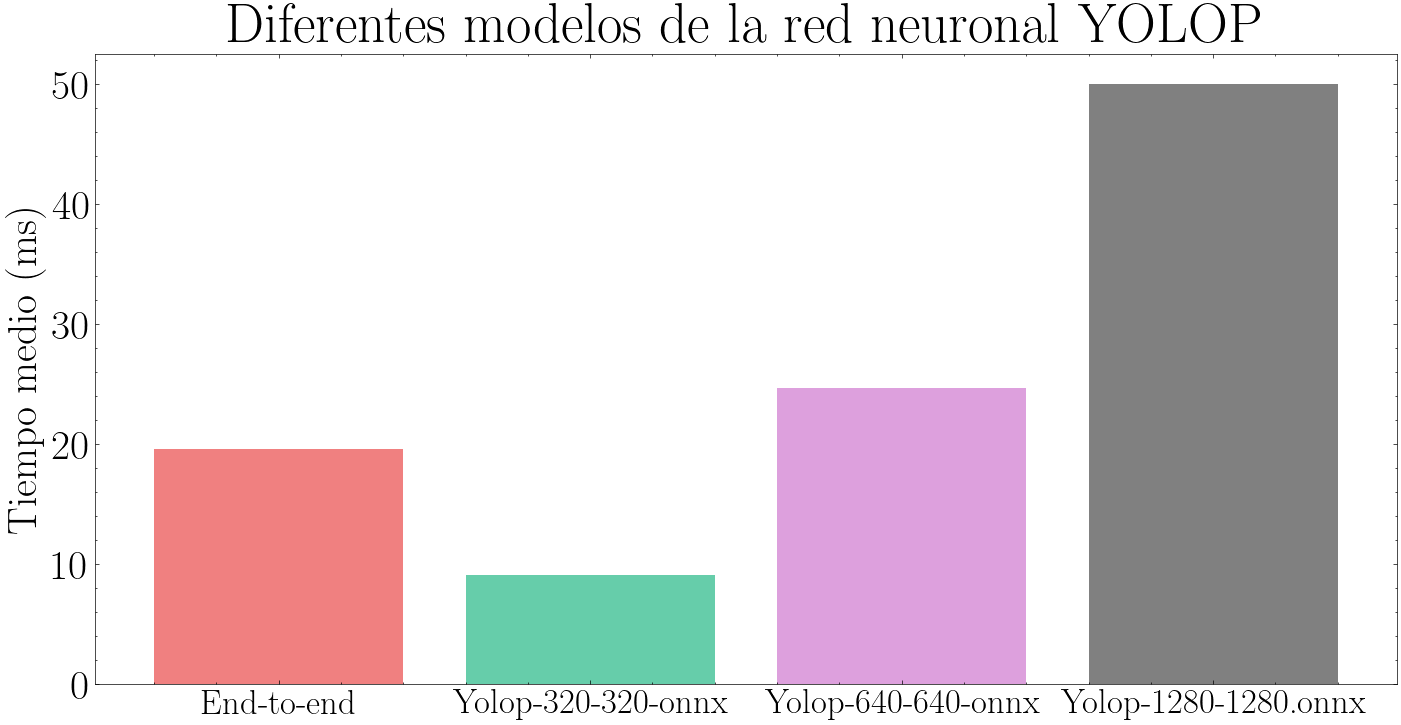
\includegraphics[scale=0.3]{figs/Diseño/YOLOP/comparativa.png}
  \end{center}
  \caption{Resultados de los diferentes modelos que ofrece la red YOLOP}
  \label{fig:resultados_pesos_preentrenados}
  \vspace{-1.5em}
\end{figure}
Por ello, se escoge el modelo \texttt{Yolop320-320.onnx} ya que obtiene mejores resultados para poder realizar la detección de las líneas del carril. 
En cuanto a los resultados de la inferencia, en la figura \ref{Proceso-YOLOP} 
se puede observar los diferentes resultados que tiene la red neuronal YOLOP dependiendo del modelo empleado. Para ello, se utilizan dos zonas totalmente distintas para realizar 
la inferencia de los modelos. Aunque se escoja el modelo \texttt{Yolop-320-320.onnx}, la detección de las líneas no es perfecta como se muestra en la figura 
\ref{f:Inferencia320-320}. Depende de como se halla entrenado la red. 
\begin{figure} [H]
  \begin{center}
    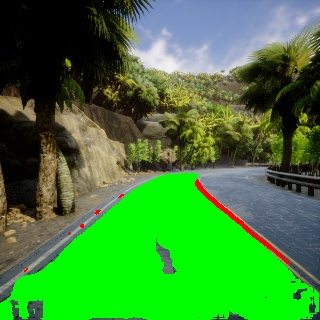
\includegraphics[scale=0.6]{figs/Diseño/YOLOP/resultados-yolop/sitio3/yolop-320-320.jpg}
  \end{center}
  \caption{Resultados de la inferencia del modelo yolop-320-320.onnx}
  \label{f:Inferencia320-320}
  \vspace{-1.5em}
\end{figure}

Para lograr una reconstrucción del carril que se desea seguir, se seleccionan las líneas que se necesitan mediante DBSCAN, un algoritmo de clustering basado en aprendizaje no supervisado. 
Con este algoritmo, se realiza una segmentación de las diferentes líneas detectadas por parte del modelo \texttt{Yolop-320-320.onnx} para más adelante aplicar un filtro y seleccionar las líneas 
para reconstruir el carril. Las líneas de la red neuronal no llegan a ser exactas, lo cual aunque se realice el filtrado de estas líneas se necesita construir el carril a partir de unas líneas 
definidas mediante regresiones cuadráticas. 
\begin{figure} [H]
  \begin{center}
    \includegraphics[scale=0.06]{figs/Diseño/YOLOP/resultados.png}
  \end{center}
  \caption{Proceso del resultado de los diferentes modelos de la red neuronal YOLOP}
  \label{Proceso-YOLOP}
\end{figure}
\newpage
\subsubsection{DBSCAN}
\label{sec:DBSCAN}

Para clasificar las lineas detectadas por parte de la red neuronal, se utiliza un algoritmo de clustering basado en aprendizaje no supervisado, en particular
DBSCAN(Density-Based Spatial Clustering of Applications with Noise)\cite{ski_dbs}.

Este algoritmo clasifica un conjunto de muestras en grupos (clústeres) basándose en la densidad de puntos en el espacio de características, que es una forma de representar
datos utilizando diferentes medidas o atributos. A diferencia de otros métodos de clustering, como K-Means\footnote{\url{https://www.iebschool.com/blog/algoritmo-k-means-que-es-y-como-funciona-big-data/}}, 
DBSCAN no requiere especificar el número de clústeres de antemano, 
siendo capaz de identificar patrones de forma arbitraria y especialmente útil para detectar estructuras complejas en los datos. 

DBSCAN requiere la configuración de varios parámetros importantes:
\begin{enumerate}
  \item \textbf{Eps}: Consiste en la distancia máxima que puede existir entre dos muestras para que una se considere vecina de la otra. Dicha distancia no se trata de un límite 
  máximo entre las distancias que puede haber dentro de un cluster. Si se elige un valor de eps muy alto, puede provocar que los clústeres distintos se combinen en el mismo grupo. 
  En cambio, un valor de eps muy pequeño puede resultar una mayor generación de clústeres pequeños.
  \item \textbf{Min\_samples}: Es el número mínimo de muestras dentro de un vecindario para que un punto se considere como un punto central incluyendo al propio punto.
  Si min\_samples se establece en un valor alto, DBSCAN encontrará clústeres más densos y 
  si el valor de min\_samples es bajo, los clústeres serán más dispersos.
  \item \textbf{Metric}: La métrica utilizada para calcular la distancia entre los conjuntos de clústeres. Por defecto se utiliza la distancia euclídea. 
\end{enumerate}

Antes de ejecutar el algoritmo, es necesario convertir la imagen resultante de la red neuronal en un array bidimensional compuesto por coordenadas de puntos x e y, por ello se utiliza
la función \texttt{column\_stack}\footnote{\url{https://numpy.org/doc/stable/reference/generated/numpy.column_stack.html}} de numpy, transformando un array
unidimensional en uno bidimensional. Cuando se realice la conversión se da pie a escoger los valores del algoritmo DBSCAN. Se ha seleccionado un valor de \texttt{eps} de 10, esto significa que, 
para que un punto sea considerado parte de un mismo clúster, debe estar a una distancia máxima de 10 píxeles para que sean vecinos y pertenezcan al mismo grupo de clúster. 
El parámetro \texttt{min\_samples} se establece en 5, al menos 5 muestras 
deben estar presentes en la vecindad de un punto para que se considere parte de un mismo clúster. 

\begin{code}[h]
  \begin{footnotesize}
  \begin{lstlisting}[language=Python]
    def clustering(self,cv_image):
    
    points_lane = np.column_stack(np.where(cv_image > 0))
    dbscan = DBSCAN(eps=10, min_samples=5,metric="euclidean")

    if points_lane.size > 0:
        dbscan.fit(points_lane)
        labels = dbscan.labels_

        clusters = set(labels)
        if -1 in clusters:
            clusters.remove(-1)
    
        for cluster in clusters:
            points_cluster = points_lane[labels==cluster,:]
            centroid = points_cluster.mean(axis=0).astype(int)
            color = self.colors[cluster % len(self.colors)]
            cv_image[points_cluster[:,0], points_cluster[:,1]] = color

        return cv_image
  
  \end{lstlisting}
  \caption[Algoritmo de clustering utilizando DBSCAN]{Algoritmo de clustering utilizando DBSCAN}
  \label{cod:DBSCAN}
  \end{footnotesize}
  \end{code}  


Al aplicar DBSCAN, el algoritmo devuelve una lista de etiquetas que van desde 0 a n, 
donde 0 representa el primer clúster detectado y n el último. Las muestras etiquetadas como ruido o no clasificadas reciben la etiqueta -1 y se eliminan de la lista de clústeres. Para visualizar 
el resultado, se itera sobre la lista de etiquetas y se muestran los puntos correspondientes de cada etiqueta en la imagen de salida. El proceso completo, incluyendo los valores 
de los parámetros de DBSCAN así como el uso de la clasificación de las líneas, se puede ver en el código \ref{cod:DBSCAN}.

La figura \ref{clasificación} se muestran los diferentes resultados que tiene este algoritmo en localizaciones distintas. En la primera fila, se muestra las imágenes originales. En la segunda 
fila se muestra el resultado del modelo \texttt{Yolop-320-320.onnx} y por último en la tercera fila se muestra el resultado de la clasificación de las líneas detectadas por la red 
utilizando el algoritmo DBSCAN. Cada clúster detectado es representado por un color distinto para poder visualizar el total de grupos que ha sido capaz clasificar DBSCAN.
Dependiendo de la ubicación del dron, DBSCAN clasifica las líneas en aproximadamente entre 3 y 4 grupos de clústeres. En función de la clasificación de DBSCAN, se realiza 
un filtrado de clústeres para seleccionar específicamente aquellos grupos de puntos que representan las líneas del carril deseado.

\begin{figure}[H]
  \centering

  % Título para la primera fila
  \textbf{Imágenes Originales}
  \vspace{0.5cm}

  \begin{minipage}[t]{0.3\textwidth}
      \centering
      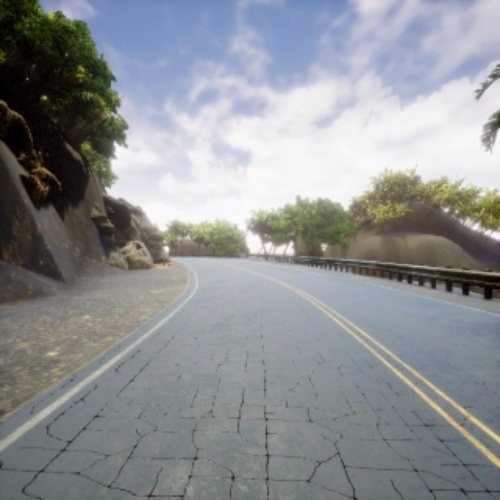
\includegraphics[width=\textwidth]{figs/Diseño/DBSCAN/comparativa/dbscan1-original.jpg}
      \caption*{}
  \end{minipage}
  \hfill
  \begin{minipage}[t]{0.3\textwidth}
      \centering
      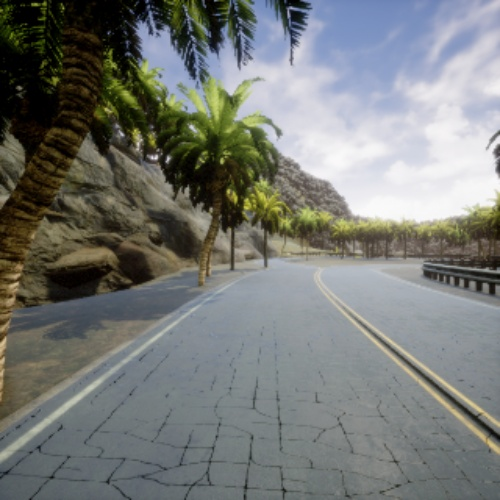
\includegraphics[width=\textwidth]{figs/Diseño/DBSCAN/comparativa/dbscan2-original.jpg}
      \caption*{}
  \end{minipage}
  \hfill
  \begin{minipage}[t]{0.3\textwidth}
      \centering
      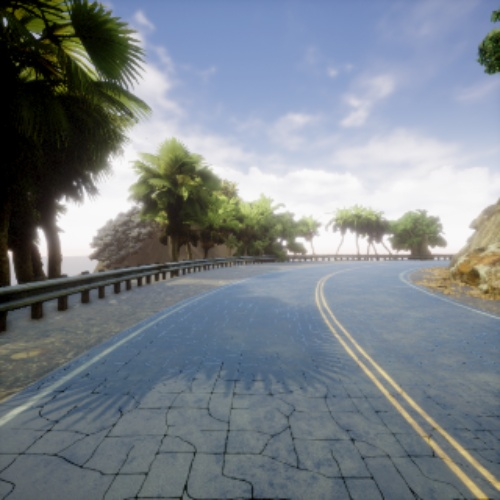
\includegraphics[width=\textwidth]{figs/Diseño/DBSCAN/comparativa/dbscan4-original.jpg}
      \caption*{}
  \end{minipage}

  \vspace{0.5cm}

  % Título para la segunda fila
  \textbf{Detección de Yolop-320-320.onnx}
  \vspace{0.5cm}

  \begin{minipage}[t]{0.3\textwidth}
      \centering
      \includegraphics[width=\textwidth]{figs/Diseño/DBSCAN/comparativa/yolop1.jpg}
      \caption*{}
  \end{minipage}
  \hfill
  \begin{minipage}[t]{0.3\textwidth}
      \centering
      \includegraphics[width=\textwidth]{figs/Diseño/DBSCAN/comparativa/yolop2.jpg}
      \caption*{}
  \end{minipage}
  \hfill
  \begin{minipage}[t]{0.3\textwidth}
      \centering
      \includegraphics[width=\textwidth]{figs/Diseño/DBSCAN/comparativa/yolop3.jpg}
      \caption*{}
  \end{minipage}

  \vspace{0.5cm}

  % Título para la tercera fila
  \textbf{Resultado de DBSCAN}
  \vspace{0.5cm}

  \begin{minipage}[t]{0.3\textwidth}
      \centering
      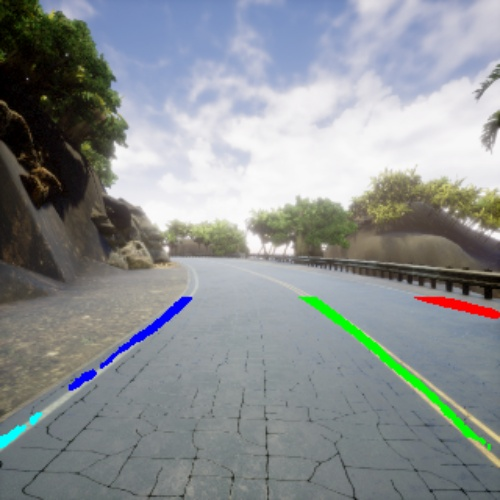
\includegraphics[width=\textwidth]{figs/Diseño/DBSCAN/comparativa/dbscan1.jpg}
      \caption*{}
  \end{minipage}
  \hfill
  \begin{minipage}[t]{0.3\textwidth}
      \centering
      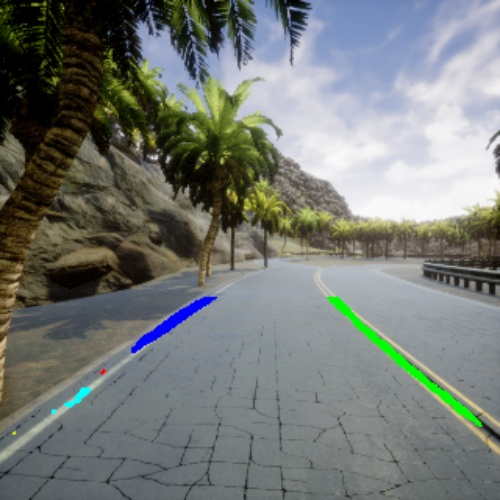
\includegraphics[width=\textwidth]{figs/Diseño/DBSCAN/comparativa/dbscan2.jpg}
      \caption*{}
  \end{minipage}
  \hfill
  \begin{minipage}[t]{0.3\textwidth}
      \centering
      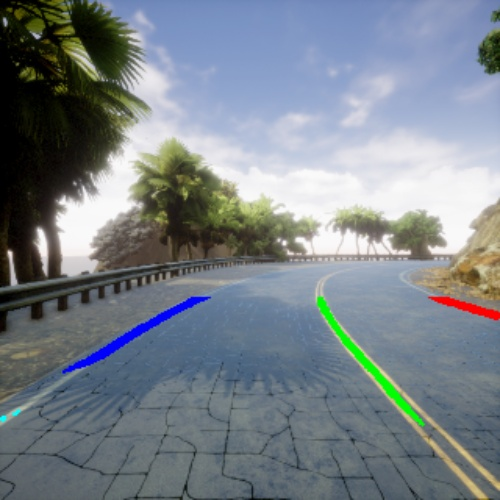
\includegraphics[width=\textwidth]{figs/Diseño/DBSCAN/comparativa/dbscan4.jpg}
      \caption*{}
  \end{minipage}

  % Caption general para la figura
  \caption{Resultado de la clasificación de las líneas por DBSCAN}
  \label{clasificación}
\end{figure}

\subsubsection{Filtrado de clústeres}
\label{clasificación:cluster}
Después de ejecutar el algoritmo DBSCAN, es crucial determinar qué grupos de clústeres pertenecen a las líneas que definen el carril que se desea seguir. 
Para lograrlo, se realiza un filtrado de los centroides de cada
grupo de clústeres detectado y se filtran según su posición respecto al centro de la imagen. La imagen tiene unas dimensiones de 320x320 píxeles, con su centro en (160,160) píxeles 
. Se consideran exclusivamente los valores horizontales de los centroides para realizar el filtrado con respecto al centro de la imagen. Basándose en este filtrado, 
los centroides se dividen en dos grupos distintos: izquierda y derecha de la imagen, como se detalla en el código \ref{cod:Clasificación de clústeres}. 

\begin{code}[h]
  \begin{lstlisting}[language=Python]
    WIDTH = cv_image.shape[1]
    if centroid[1] < WIDTH/2:  # left lane
        left_clusters.append((points_cluster,centroid))
       
    elif centroid[1] >= WIDTH/2:  # right lane
        right_clusters.append((points_cluster, centroid))
  \end{lstlisting}
  \caption[Clasificación de clústeres según las dimensiones de la imagen ]{Clasificación de clústeres respecto a las dimensiones de la imagen}
  \label{cod:Clasificación de clústeres}
  \end{code}  

Durante el proceso de filtrado de los grupos de clústeres, se seleccionan subgrupos específicos de cada grupo (izquierda y derecha). Los subgrupos se eligen utilizando una función 
maximizada con respecto a un punto central predefinido P, cuyo valor es (160,220), ajustado según las dimensiones de la imagen de 320x320 píxeles . El resto de clústeres son 
descartados. Esta función maximizada se detalla en el código \ref{cod:funcion_maximizada}. 

Al manipular puntos en numpy, es importante recordar que las coordenadas están invertidas (y,x en lugar de x,y). Además de seleccionar subgrupos en relación con el punto central P, 
se considera también la densidad de puntos en los grupos de clústeres detectados tanto en la izquierda como en la derecha. Este enfoque garantiza que la selección no solo dependa 
de la proximidad al punto central, sino también de la cantidad de puntos presentes.
\begin{code}[h]
  \begin{lstlisting}[language=Python]
    def score_cluster(self,cluster, center):
      points_cluster, centroid = cluster
    
      proximity = np.linalg.norm(centroid - center)
      density = len(points_cluster)
      return density / proximity

  \end{lstlisting}
  \caption[Función maximizada para escoger el grupo de cluster más cercano y denso respecto al punto P]{Función maximizada para escoger el grupo de clúster más cercano y denso respecto al punto P}
  \label{cod:funcion_maximizada}
  \vspace{-1.5em}
  \end{code}  
 
  En la figura \ref{fig:comparativa} se muestra el proceso desde la clasificación de líneas por DBSCAN hasta la selección de los clústeres. 
  DBSCAN es capaz de detectar hasta 4 clústeres, a partir de los cuales se realiza un filtrado basado en las coordenadas x de cada centroide de cada clúster. Posteriormente, 
  se aplica una función maximizada para obtener los 2 clústeres requeridos. Estos clústeres están representados en color rojo para el grupo izquierdo y en verde para el grupo 
  derecho. 
  \begin{figure}[H]
    \centering
    \begin{minipage}{0.3\textwidth}
      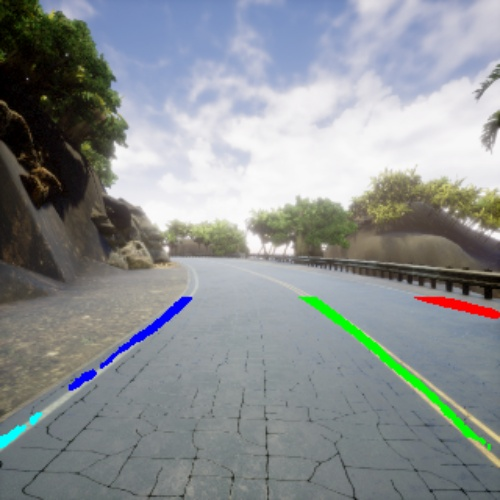
\includegraphics[width=\linewidth]{figs/Diseño/DBSCAN/comparativa/dbscan1.jpg}
    \end{minipage}
    \hfill
    \begin{minipage}{0.3\textwidth}
      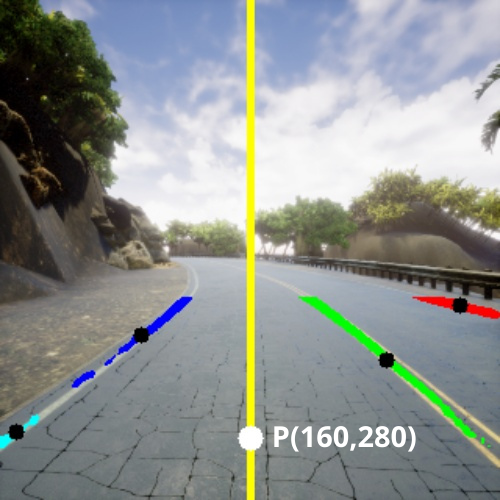
\includegraphics[width=\linewidth]{figs/Diseño/DBSCAN/clustering_centroids.png}
    \end{minipage}
    \hfill
    \begin{minipage}{0.3\textwidth}
      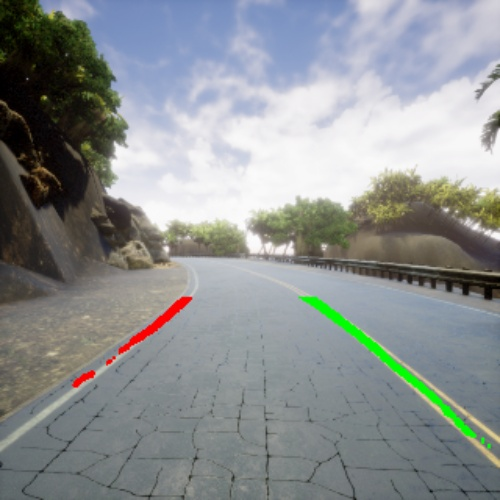
\includegraphics[width=\linewidth]{figs/Diseño/DBSCAN/filter_clustering.jpg}
    \end{minipage}
    \caption{Proceso de filtrado de las líneas clasificadas por DBSCAN}
    \label{fig:comparativa}
  \end{figure}

\subsubsection{Regresión cuadrática}
\label{sec:Regresión cuadrática}
Al tener los clústeres seleccionados, es necesario construir dos líneas que representen la naturaleza del carril basándose en estos puntos. Para ello, se emplea una técnica de aprendizaje 
automático conocida como regresión, que permite aproximar a un número N de puntos a una recta, curva u otra forma matemática que se pueda definir con una función. 
Debido a que las líneas de los carriles rara vez son 
completamente rectas, suelen ser curvilíneas, se opta por utilizar una regresión de tipo cuadrática. 

La regresión cuadrática permite modelar los puntos de cada clúster como curvas, lo cual es más adecuado para capturar las variaciones y curvaturas típicas de los carriles. Esta técnica no solo
ayuda a interpretar mejor la forma del carril, sino que también facilita la navegación del dron al seguir la trayectoria por el carril.

Para la construcción de las regresiones cuadráticas se utiliza las funciones de la librería numpy denominada \texttt{Polyfit}\footnote{\url{https://numpy.org/doc/stable/reference/generated/numpy.polyfit.html}}
y \texttt{Polyval}\footnote{\url{ https://numpy.org/doc/stable/reference/generated/numpy.polyval.html}}. 
\texttt{Polyfit} es una función que calcula los coeficientes del polinomio que mejor se ajusta a los datos utilizando el método de los mínimos 
cuadrados para la ecuación cuadrática, obteniendo tres coeficientes, denominados a, b y c. Se define los valores de las coordenadas x como los puntos que se quiere
realizar dicho calculo, se realiza un rango entre un mínimo y un máximo ajustándolo a las dimensiones de la imagen, además de la ayuda de 
dos puntos auxiliares en los extremos inferiores en el cálculo de la regresión, esto se realiza para que la regresión cuadrática tienda a las esquinas superiores de la imagen 
como se muestra en el código \ref{cod:Calculocoeficientes}.
 

\begin{code}[H]
  \begin{lstlisting}[language=Python]
  
    FACTOR_PIXEL = 20
    MIN_VALUE_X = (cv_image.shape[1] // 2) + FACTOR_PIXEL
    MAX_VALUE_X = cv_image.shape[1]
  
    valuesX = np.arange(MIN_VALUE_X,MAX_VALUE_X) 
    point = np.array([cv_image.shape[1]/1.104,cv_image.shape[1]])
    coefficients = np.polyfit(points_cluster[:,0],points_cluster[:,1],2)
  \end{lstlisting}
  \caption[Calculo de los coeficientes]{Cálculo de los coeficientes de la regresión cuadrática}
  \label{cod:Calculocoeficientes}
  \vspace{-1.5em}
  \end{code}  
Se realiza un promedio de los últimos diez valores utilizando los coeficientes mencionados, como se ilustra en el código \ref{cod:regresión}. Este promedio se recalcula 
cada cinco iteraciones. Este paso es crucial para reducir las oscilaciones causadas por las detecciones de la red neuronal, las cuales son fundamentales para el comportamiento sigue-carril. Una vez calculados los 
coeficientes, se calcula la regresión cuadrática mediante la función \texttt{Polyval}, dicha función calcula
la función cuadrática con los coeficientes calculados anteriormente. 

Al obtener los valores de la función cuadrática, se seleccionan los puntos de dicha función que se encuentran en el eje y, entre 0 y el máximo de la imagen menos uno (es decir, entre 0 y 319). 
Este proceso se debe realizar debido a que el resultado de la función \texttt{Polyval} puede dar como resultado números negativos. En una imagen no se puede indexar con números negativos ya que 
se corresponderían a píxeles que se encuentran fuera de la propia imagen.

Este proceso se realiza dos veces, una regresión cuadrática para el grupo de clústeres detectados escogidos de la derecha y otra regresión cuadrática para el grupo de clústeres detectados
escogidos de la izquierda. 
Finalmente, con dichas regresiones cuadráticas se procede a realizar una dilatación de los puntos para tener un resultado más llamativo y visual al poder
ver las regresiones cuadráticas. El resultado se puede visualizar en la figura \ref{fig:regresión cuadrática} teniendo presente los pasos que se ha tenido que seguir para 
realizar las regresiones, dichas líneas se representan de color amarillo.

\begin{code}[H]
  \begin{lstlisting}[language=Python]

    self.list_coeff_a.append(coefficients[0])
    self.list_coeff_b.append(coefficients[1])
    self.list_coeff_c.append(coefficients[2])

    a = np.mean(self.list_coeff_a[-10:])
    b = np.mean(self.list_coeff_b[-10:])
    c = np.mean(self.list_coeff_c[-10:])

    mean_coeff = np.array([a,b,c])

    self.counter += 1

    if(self.counter > 5):
      self.list_coeff_a.clear()
      self.list_coeff_b.clear()
      self.list_coeff_c.clear()  


    values_fy = np.polyval(mean_coeff,valuesX).astype(int)
    fitLine_filtered = [(x, y) for x, y in zip(valuesX, values_fy) if 0 <= y <= (cvimage.shape[1] - 1)]
    line = np.array(fitLine_filtered)
   

  \end{lstlisting}
  \caption[Cálculo de la regresión cuadrática]{Cálculo de la regresión cuadrática}
  \label{cod:regresión}
  \end{code}  
\begin{figure} [H]
  \begin{center}
    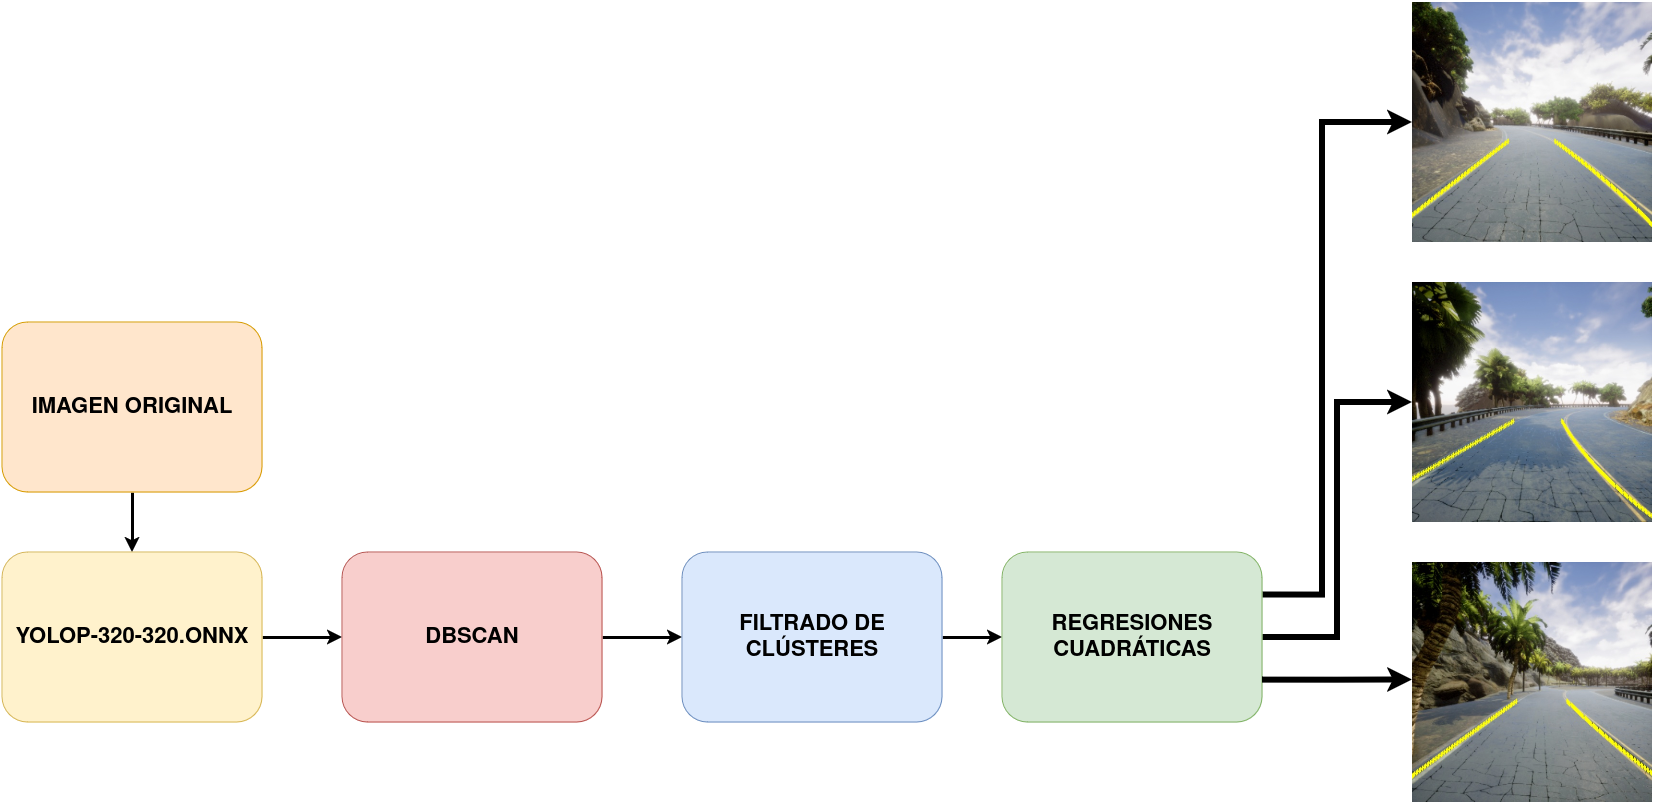
\includegraphics[scale=0.28]{figs/Diseño/Regresiones/regresiones.png}
  \end{center}
  \caption{Resultado de la regresión cuadrática}
  \label{fig:regresión cuadrática}
\end{figure}

\subsubsection{Interpolación y cálculo del centro de masas del carril}
\label{sec:Interpolación y cálculo del centro de masas del carril}

Una vez obtenidas las líneas reconstruidas, se necesita definir el área de carril dentro de estas líneas. Como se menciona en la sección 
\ref{sec:resultados}, los resultados del modelo \texttt{Yolop-320-320.onnx} respecto al área del carril no son totalmente exactos produciéndose una mala detección por parte de la red. Por lo tanto, se requiere
una técnica para construir el área del carril a partir de las líneas obtenidas mediante regresiones cuadráticas. Por ello, se utiliza una interpolación para recorrer y calcular los puntos que se encuentran
dentro de los límites de las regresiones.

Se realizan dos interpolaciones, una para 
los puntos de la regresión de la  derecha
y otra para los puntos de la regresión izquierda. 


\begin{code}[h]
  \begin{lstlisting}[language=Python]

    def interpolate_lines(self,cvimage,points_line_left,points_line_right):

    gray_image = cv2.cvtColor(cvimage, cv2.COLOR_BGR2GRAY) 
    np_gray = np.array(gray_image)
    x, y = np.nonzero(np_gray)
    img_points = np.column_stack((x, y))

    f1 = interp1d(points_line_left[:, 0], points_line_left[:, 1],kind='slinear',fill_value="extrapolate")
    f2 = interp1d(points_line_right[:, 0], points_line_right[:, 1],kind='slinear',fill_value="extrapolate") 
    y_values_f1 = f1(img_points[:, 0])
    y_values_f2 = f2(img_points[:, 0])
    indices = np.where((y_values_f1 < img_points[:, 1]) & (img_points[:, 1] <= y_values_f2))
    
    points_between_lines = img_points[indices]
    filtered_points_between_lines = points_between_lines[points_between_lines[:,0] > 180]
    return filtered_points_between_lines
    
  \end{lstlisting}
  \caption[Método de interpolación]{Método del cálculo de las funciones de interpolación}
  \label{cod:interpolación}
  \end{code}  

Estas funciones interpolan los valores de los puntos en \textit{y} en función de los valores de los puntos en \textit{x}, 
más adelante se evalúa los valores de los puntos que se encuentran entre 
ambas regresiones cuadráticas como se muestra en el código \ref{cod:interpolación}. Cuando se proceda a dicha evaluación, se desarrolla un filtro 
para seleccionar un fragmento de carril. El carril se representa en color azul en la imagen resultante.

En la figura \ref{comparativa-interpolacion}, se contrasta los resultados obtenidos por parte del modelo \texttt{Yolop-320-320.onnx} y la construcción del carril calculada a partir de las regresiones. 
Como se puede observar, la construcción del carril desarrollada es bastante robusta en comparación con la salida que te ofrece la red, siendo así una forma de poder construir un 
carril. Finalmente, para poder realizar el comportamiento sigue-carril, el dron necesita mantener una alineación respecto al carril calculado, por ello 
se calcula el centro de masas que tiene el carril.

Para el cálculo del centroide del carril, se toma ecuación \ref{eq:funcioncentromasas}, que consiste en el cálculo de centro de masas de una superficie. 
  \begin{myequation}[h]
    \begin{equation} 
      \vec{r}_{CM} = \frac{\sum_{i}m_{i} \vec{r}_{i}}{\sum_{i}m_{i}} = \frac{\sum_{i}m_{i} \vec{r}_{i}}{M} 
      \label{eq:funcioncentromasas}
    \end{equation} 
    \caption{Calculo del centro de masas}
    \vspace{-1.5em}
  \end{myequation}

  Siendo $\vec{r}_{CM}$ las coordenadas del centroide compuesta por (x,y), $\vec{r}_{i}$ los puntos del carril construido y $m_{i}$ la masa que constituye cada punto, se supone que todos 
  los puntos del carril tienen masa igual a 1. Dicha suposición, simplifica el cálculo, pero en aplicaciones del mundo real, las masas pueden variar. 

\begin{figure}[H]
  \centering

  % Título para la primera fila
  \textbf{Detección de Yolop-320-320.onnx}
  \vspace{0.5cm}

  \begin{minipage}[t]{0.2\textwidth}
      \centering
      \includegraphics[width=\textwidth]{figs/Diseño/Regresiones/yolop1.jpg}
      \caption*{}
  \end{minipage}
  \hfill
  \begin{minipage}[t]{0.2\textwidth}
      \centering
      \includegraphics[width=\textwidth]{figs/Diseño/Regresiones/yolop2.jpg}
      \caption*{}
  \end{minipage}
  \hfill
  \begin{minipage}[t]{0.2\textwidth}
      \centering
      \includegraphics[width=\textwidth]{figs/Diseño/Regresiones/yolop3.jpg}
      \caption*{}
  \end{minipage}
  \hfill
  \begin{minipage}[t]{0.2\textwidth}
      \centering
      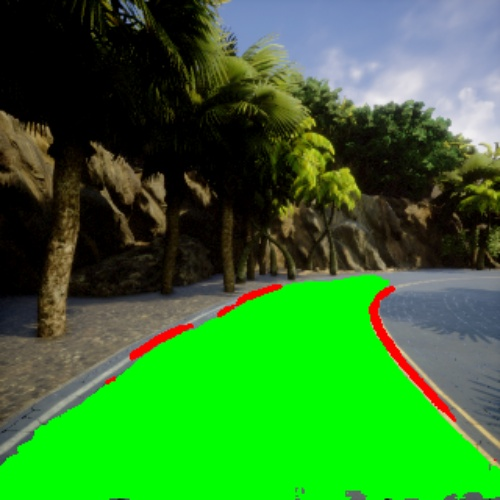
\includegraphics[width=\textwidth]{figs/Diseño/Regresiones/yolop4.jpg}
      \caption*{}
  \end{minipage}

  \vspace{0.5cm}

  % Título para la segunda fila
  \textbf{Construcción del carril desarrollada}
  \vspace{0.5cm}

  \begin{minipage}[t]{0.2\textwidth}
      \centering
      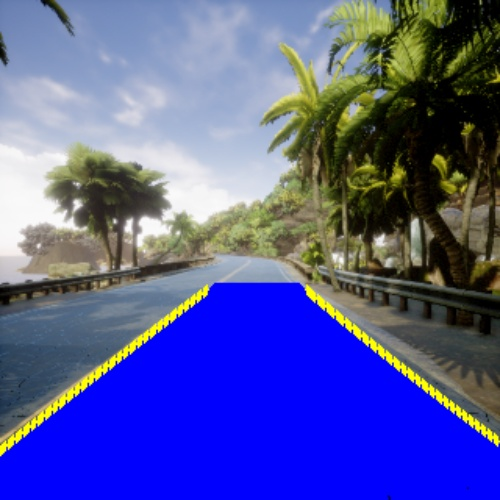
\includegraphics[width=\textwidth]{figs/Diseño/Regresiones/interpolación1.jpg}

  \end{minipage}
  \hfill
  \begin{minipage}[t]{0.2\textwidth}
      \centering
      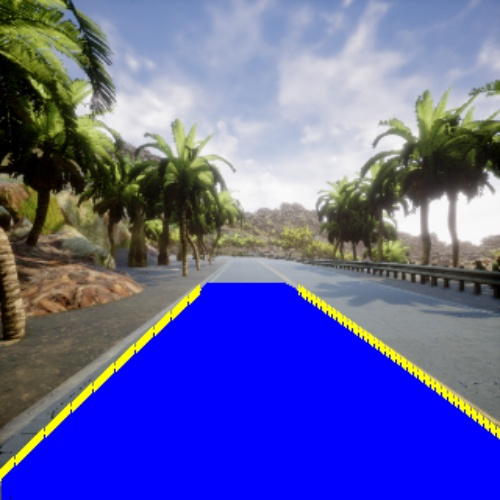
\includegraphics[width=\textwidth]{figs/Diseño/Regresiones/interpolación2.jpg}
  \end{minipage}
  \hfill
  \begin{minipage}[t]{0.2\textwidth}
      \centering
      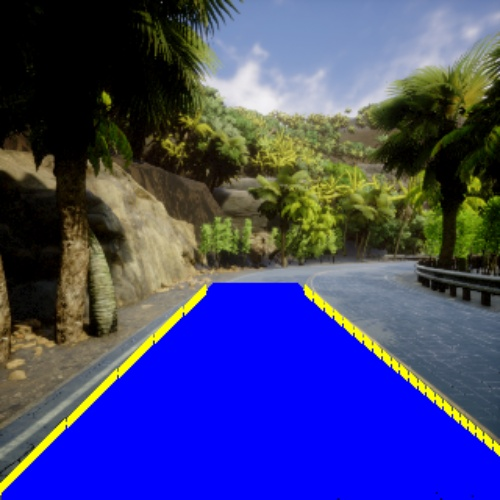
\includegraphics[width=\textwidth]{figs/Diseño/Regresiones/interpolación3.jpg}
  \end{minipage}
  \hfill
  \begin{minipage}[t]{0.2\textwidth}
      \centering
      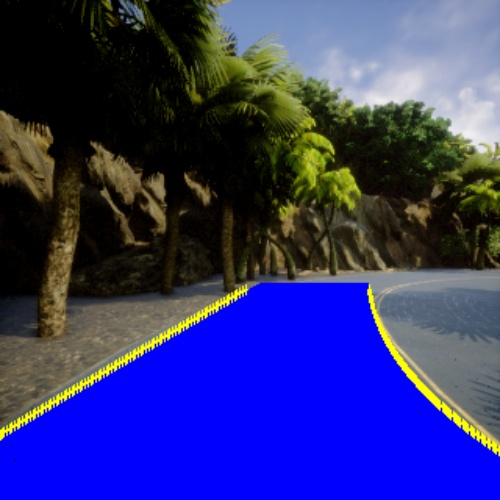
\includegraphics[width=\textwidth]{figs/Diseño/Regresiones/interpolación4.jpg}
  \end{minipage}
  % Caption general para la figura
  \caption{Comparativa entre el resultado de detección Yolop-320-320.onnx y la construcción del carril desarrollada}
  \label{comparativa-interpolacion}
  \vspace{-1.5em}
\end{figure}
  El cálculo de masa total ($\sum_{i}m_{i} \vec{r}_{i}$), consiste en el producto entre la masa individual de cada punto por el tamaño de los puntos que componen el carril. A continuación, 
  se realiza el sumatorio de las coordenadas de los puntos ponderados por su masa y la división por el cálculo de masa total. El resultado de la ecuación es el conocido centroide 
  compuesto por (x,y).
  
  El resultado final del cálculo del centroide se muestra en la figura \ref{fig:centro de masas} resaltando con una flecha de color rojo donde se encuentra
  el centro de masas del carril representado por un círculo de color blanco. Este centroide se utilizará en los controladores que se explicarán
  posteriormente, para poder determinar que tan desviado esta el dron respecto al centro del carril, que se representa con este centro de masas.

  \begin{figure} [H]
    \begin{center}
      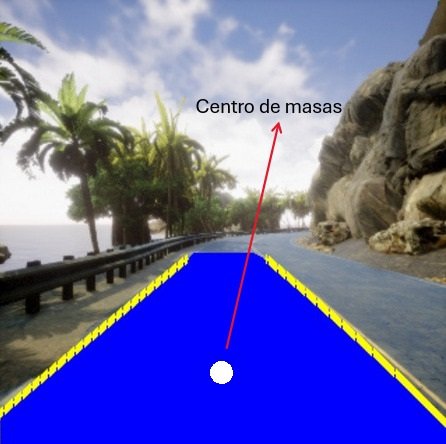
\includegraphics[scale=0.6]{figs/Diseño/Regresiones/centroide.jpeg}
    \end{center}
    \caption{Resultado del centro de masas}
    \label{fig:centro de masas}
    \vspace{-1.5em}
  \end{figure}

  \subsection{Análisis del algoritmo de percepción}
  \label{sec:Análisis del algoritmo de percepción}
  A continuación, se realiza un análisis detallado de cada submódulo del sistema perceptivo. Esta evaluación se presenta en la tabla \ref{tab:Profiling}, incluye 
  tres columnas indicando el nombre  de cada componente del sistema perceptivo, el dispositivo donde se ejecuta y el tiempo medio calculado en milisegundos.

\begin{table}[h]
    \centering
    \begin{tabular}{| m{5cm} | m{3cm} | m{3cm} |}
        \hline
        \textbf{Componentes Percepción} & \textbf{Dispositivo} & \textbf{Tiempo (ms)} \\ \hline
        YOLOP & GPU & 9.523 \\ \hline
        Procesamiento de YOLOP & CPU & 0.195 \\ \hline
        DBSCAN & CPU & 0.000301 \\ \hline
        Filtrado de clústeres & CPU & 6.867 \\ \hline
        Regresiones cuadráticas & CPU & 3.593 \\ \hline
        Interpolación & CPU & 8.532 \\ \hline
        Cálculo del centro de masas & CPU & 0.0427 \\ \hline
        \textbf{Tiempo Total} & & \textbf{28.753} \\ \hline
    \end{tabular}
    \caption{Profiling}
    \label{tab:Profiling}
\end{table}

Estos datos se recopilan utilizando un ordenador portátil (PC2) con una GPU Nvidia RTX 2070, como se menciona en la sección de arquitectura. La tabla muestra que los 
componentes perceptivos que requieren más tiempo de procesamiento son la inferencia del modelo \texttt{Yolop-320-320.onnx} y el cálculo de las interpolaciones. 
Aunque la inferencia se realiza en la GPU, está constantemente procesando imágenes para generar la salida. Por otro lado, la interpolación 
requiere procesar todos los puntos que pertenecen a las dos regresiones, lo cual consume recursos de la CPU.

En comparación, el componente DBSCAN es el más eficiente en términos de tiempo de cómputo, lo que hace interesante trabajar con este algoritmo de clustering. 
Sumando los tiempos de cada componente, se obtiene un tiempo medio total de 28.753 milisegundos, lo que se traduce en un procesamiento aproximado de 30 FPS (frames por segundo). 

Este análisis es crucial para conseguir un sistema perceptivo en tiempo real a la hora de implementar los comportamientos de control. 

  \section{Comportamientos de control}
  \label{sec:Control}

  En este sub-apartado, se describe el desarrollo de los comportamientos de control junto con el sistema perceptivo desarrollado para posteriormente realizar 
  una comparativa entre ambos y contrastar los resultados obtenidos.

\subsection{Sigue-carril basado en PID}
\label{sec:Control-PID}

A partir del sistema perceptivo, se desarrolla un comportamiento autónomo de sigue-carril utilizando un controlador PID. Este comportamiento tiene como objetivo
demostrar la efectividad del sistema perceptivo y la capacidad del dron para mantenerse centrado y corregir desviaciones en relación
con el centroide del carril en tiempo real. El controlador PID ajusta continuamente las velocidades angulares del dron para mantener un ángulo lo más alineado posible respecto con el
centro del carril, reduciendo así el error de desviación.

El proceso de ajuste de las constantes del controlador PID es crucial y debe realizarse de manera iterativa, adaptándose a las condiciones específicas del entorno. Es importante
destacar que los valores óptimos de las constantes para un escenario particular pueden no ser aplicables directamente a otros escenarios, lo que requiere ajustes personalizados. 
En cuanto a la velocidad lineal, se mantiene un valor constante.

Además del controlador PID utilizado para el seguimiento del carril, se implementa otro controlador PD para mantener la altura del dron con respeto al suelo durante su navegación. 
Esto se debe a la naturaleza del simulador, donde las carreteras presentan variaciones en su elevación, lo que puede afectar la detección del carril del sistema perceptivo. Por lo cual, 
con este controlador PD, permite al dron ajustar su altitud, asegurando así una altura constante y estable. En el código \ref{cod:ValoresPID} se expone los valores de cada 
constante de los controlador PID Y PD ajustadas.

En la figura \ref{sigue-carril}, se muestran diferentes frames de la navegación autónoma 
del dron utilizando el controlador anteriormente descrito. En las imágenes
se muestran los valores de la velocidad lineal, angular, el error con respecto al centro de masas y una línea representando la mitad de la imagen. 
En la primera imagen y en la segunda, el error se encuentra
entre 4 y 7 píxeles, mostrando que el dron consigue una alineación centrada respecto al carril. Por último, en la tercera imagen 
se muestra una desviación significativa con un error de 16 píxeles, el controlador
PID realiza ajustes en la velocidad angular para corregir la trayectoria. 

\begin{figure}[H]
  \centering
  \begin{minipage}[t]{0.3\textwidth}
      \centering
      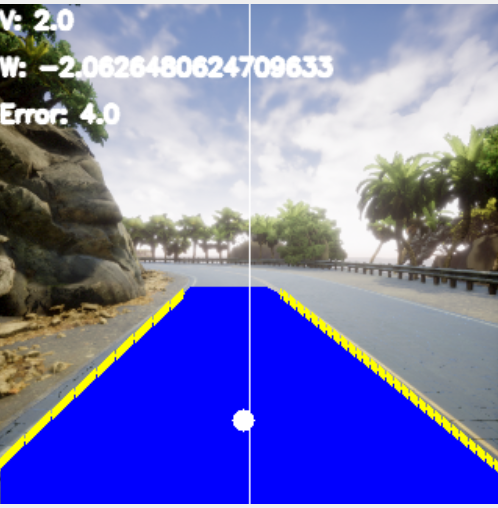
\includegraphics[width=\textwidth]{figs/Diseño/PID/PID1.png}
  \end{minipage}
  \hfill
  \begin{minipage}[t]{0.3\textwidth}
      \centering
      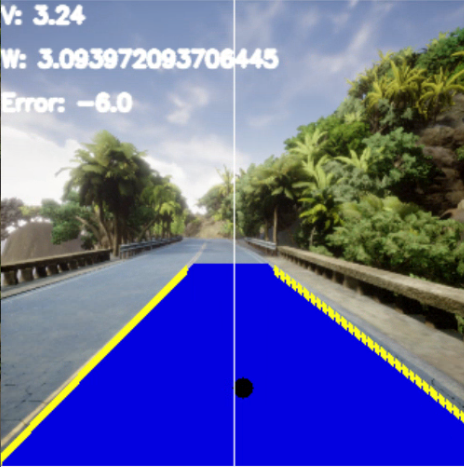
\includegraphics[width=\textwidth]{figs/Diseño/PID/PID2.png}
  \end{minipage}
  \hfill
  \begin{minipage}[t]{0.3\textwidth}
      \centering
      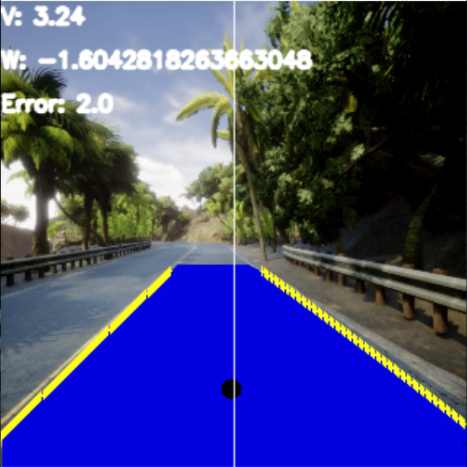
\includegraphics[width=\textwidth]{figs/Diseño/PID/PID3.png}
  \end{minipage}
  \caption{Sigue-carril basado en PID}
  \label{sigue-carril}
  \vspace{-1.5em}
\end{figure}

  \begin{code}[h]
    \begin{lstlisting}[language=Python]

      kp_height = 0.1
      kd_height = 0.4

      kp_speed_controller = 0.09
      kd_speed_controller = 0.1
      ki_speed_controller = 0.008
     
    \end{lstlisting}
    \caption[Valores de las variables del PD del control de altura y del PID del controlador de velocidad angular]{Valores de las variables del PD del control de altura y del PID del controlador de velocidad angular}
    \label{cod:ValoresPID}
    \end{code} 

   

Este controlador PID, aunque funcional, presenta problemas ya que es incapaz de adaptarse a todos los escenarios, ya que en algunos casos más complicados en los que las curvas son más cerradas
el controlador es incapaz de trazar la curva provocando una salida de carril por parte del dron. 

Debido a esto, se considera una implementación de técnicas de aprendizaje por refuerzo. Estas técnicas, 
permiten al dron aprender y adaptarse de manera autónoma a diversas condiciones del entorno, manteniéndose centrado en el carril de manera más eficiente y robusta en comparación 
con los métodos de control tradicionales. Este método a diferencia del anterior, permite al dron generalizar las acciones que debe de tomar ante distintas situaciones del entorno, lo que tiene
como consecuencia que este pueda funcionar correctamente ante entornos desconocidos.
  \subsection{Sigue-carril basado en aprendizaje por refuerzo}
  \label{sec:aprendizaje por refuerzo}

  Como se menciona en la sección \ref{sec:IA}, el aprendizaje por refuerzo consiste en enseñar a un agente a
  desempeñar un comportamiento deseado mediante recompensas y penalizaciones. Este comportamiento se aprende a base de interacciones con el entorno de trabajo y observaciones de como puede responder,
  de forma similar a los niños que exploran el mundo que les rodea y aprenden las acciones que les ayudan a alcanzar un objetivo. 

  En este TFG se emplea como algoritmo de aprendizaje por refuerzo, el algoritmo Q-learning. Este se basa en una tabla de correspondencias estado-acción que almacena ante distintos estados 
  la acción que se debe de tomar para maximizar la recompensa. Para este algoritmo es necesario definir distintos componentes, que son: agente, entorno, estados, acciones, función de recompensa y 
  la política.
  
  Los componentes del algoritmo Q-learning, que se definen para la tarea del sigue-carril son los siguientes: 
  \begin{itemize} 
    \item \textbf{Agente}: En este caso, el dron. Es la entidad o modelo que se pretende entrenar para que aprenda a tomar decisiones (acciones) en función del estado en el que se 
    encuentre y de las observaciones que vea en el entorno. 
    
    \item \textbf{Entorno}: El dron interactuará con el entorno de simulación Airsim, específicamente en el mapa Coastline, durante su navegación, aprendiendo el comportamiento deseado.

    \begin{figure} [H]
      \begin{center}
        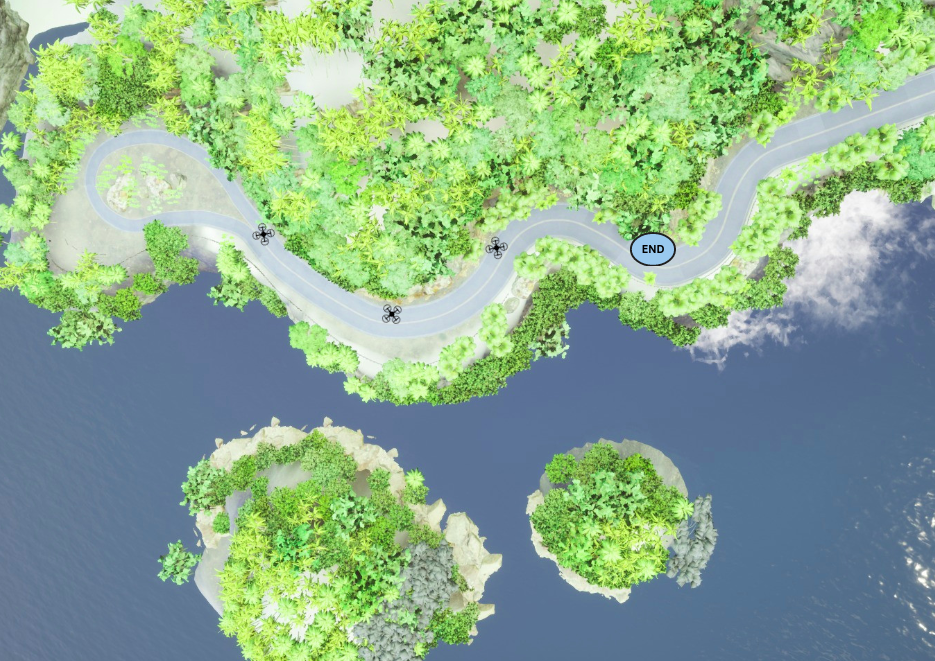
\includegraphics[scale=0.4]{figs/Diseño/RL/entorno.png}
      \end{center}
      \caption{Entorno en la fase de entrenamiento del sigue carril basado en Q-Leaning}
      \label{fig:Entorno}
      \vspace{-1.5em}
    \end{figure}

    Dentro de este escenario, se ha considerado tres localizaciones distintas para el dron a la hora de realizar el entrenamiento, así como un punto final del recorrido, como se muestra en la figura
    \ref{fig:Entorno}. La idea de utilizar diferentes localizaciones de inicio es evitar que el modelo haga sobreajuste (overfitting)\footnote{\url{https://iartificial.blog/aprendizaje/estrategias-para-evitar-el-overfitting-en-modelos-de-ml/}} 
    , es decir, que se aprenda de memoria los movimientos que debe hacer, para completar la ruta. En su lugar, se quiere que el dron 
    sea capaz de aprender y adaptarse a diversas situaciones, desarrollando así un comportamiento más generalizado y robusto. Esto se consigue debido a que en los distintos 
    entrenamientos, para una misma iteración, el dron se encontrará en posiciones distintas de la carretera, ya que la posición de inicio se elige de forma aleatoria (equiprobable) para cada
    episodio.
    
    \item \textbf{Estados}: Se necesita definir las situaciones que se puede encontrar el dron navegando dentro  por el carril. Por ello, se divide verticalmente la imagen del sistema perceptivo
    en múltiples franjas representando cada una franja un estado. En total son 14 franjas equidistantes de 10 píxeles, empezando desde la izquierda de la imagen hasta la derecha. La determinación
    del estado actual del dron se basa en las coordenadas en píxeles que se encuentra ubicado el centro de masas del carril calculado. Se puede observar el 
    resultado de los estados en la figura \ref{fig:Estados}. En total se definen 15 estados.
    
    \begin{figure} [H]
      \begin{center}
        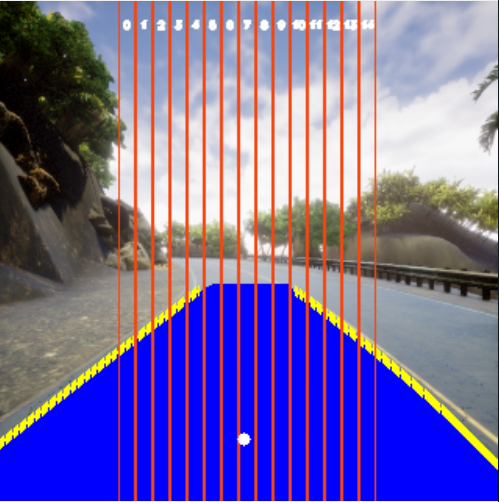
\includegraphics[scale=0.5]{figs/Diseño/RL/Estados.png}
      \end{center}
      \caption{Estados definidos para el sigue-carril basado en aprendizaje por refuerzo}
      \label{fig:Estados}
      \vspace{-1.5em}
    \end{figure}

    \item \textbf{Acciones}: En total, se han definido 21 acciones que el agente puede llevar a cabo. Se componen de pares de velocidades lineales y angulares, las velocidades lineales
    tienen un intervalo de 0.1 m/s hasta 2.0 m/s. Así siendo el intervalo de la velocidad angular de -25 hasta 25 grados/segundo, teniendo giros hacia la izquierda y hacia la derecha. Dichos pares
    de velocidades estan formados a partir de la función que nos proporciona numpy llamada \texttt{linspace}\footnote{\url{https://numpy.org/doc/stable/reference/generated/numpy.linspace.html}}. 

    En la figura \ref{fig:Acciones}, se puede observar las acciones definidas en 3 partes. En color naranja se representa las acciones con giro izquierdo, en color rojo se presenta 
    la acción central definida así como velocidad lineal sin velocidad angular y en color azul, las acciones con giro derecho. Cada pareja de acción tiene un identificador, desde el 0
    siendo la primera acción hasta el 20 siendo la última acción.
  
    \begin{figure} [H]
      \begin{center}
        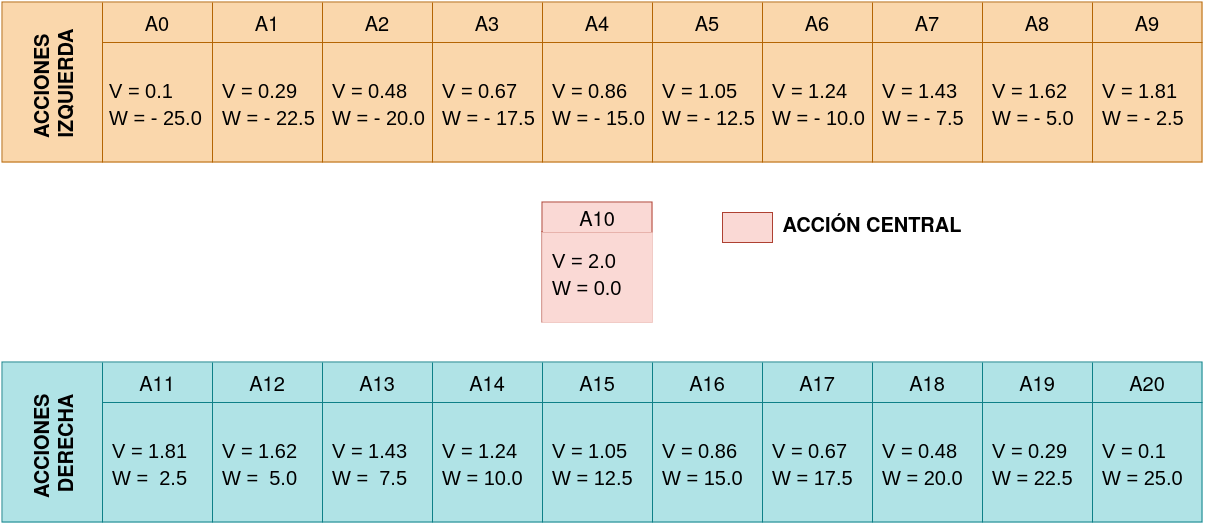
\includegraphics[scale=0.28]{figs/Diseño/RL/Tabla_acciones.png}
      \end{center}
      \caption{Acciones disponibles para el sigue-carril basado en aprendizaje por refuerzo}
      \label{fig:Acciones}
      \vspace{-1.5em}
    \end{figure}
  
    \item \textbf{Función de Recompensa o Penalizaciones}: Determina cómo se premia o penaliza el agente para que alcance el objetivo deseado. Las recompensas o penalizaciones
    se definen en una función específica, la cual varía según el objetivo que se quiere lograr. La función de recompensa se compone en dos partes: premiar al dron por permanecer 
    centrado en el carril y premiarlo por mantener una orientación adecuada con respecto al carril. 

    Cada parte de la función tiene un peso de importancia diferente: un 85\% por permanecer centrado en el carril y un 15\% para la orientación respecto al carril. Ambas partes 
    son normalizadas en un rango de 0 a 1. Además, se penaliza con un valor constante de -10 al dron cuando se sale del carril o pierde la percepción. En la ecuación 
    \ref{eq:funcionrecompensa} se muestra las dos componentes descritas, siendo $norm(error_{centro})$ y $norm(error_{angulo})$ las normalizaciones del error del centro de 
    masas del carril y la orientación, respectivamente, multiplicadas por sus pesos correspondientes.

      \begin{myequation}[H]
        \begin{equation}
          R(s,a) = (1 - norm(error_{centro})) \cdot w_{1} + 
          (1 - norm(error_{angulo})) \cdot w_{2}
          \label{eq:funcionrecompensa}
        \end{equation}
        \caption{Función de recompensa}
      \end{myequation}

   
    \begin{code}[H]
      \begin{lstlisting}[language=Python]
  
        def reward_function(self,cx,angle):

        reward = 0
        target_heading = 0
        error_lane_center = (WIDTH/2 - cx)
        heading_difference = (target_heading - angle) 
        
        MIN_ERROR = 0
        MAX_ERROR = 80

        MIN_ANGLE = 0
        MAX_ANGLE = 70

        CENTRE_WEIGHT = 0.85
        ANGLE_WEIGHT = 0.15
        
        if (self.is_exit_lane(cx)):
            reward = -10

        else:
            normalise_error_centre = (abs(error_lane_center) - MIN_ERROR) / (MAX_ERROR - MIN_ERROR)
            reward_centre = 1 - normalise_error_centre

            
            normalise_error_angle = (abs(heading_difference) - MIN_ANGLE) / (MAX_ANGLE - MIN_ANGLE)
            reward_angle = 1 - normalise_error_angle

            reward = (reward_centre * CENTRE_WEIGHT) + (reward_angle * ANGLE_WEIGHT)
            
        return reward
       
      \end{lstlisting}
      \caption[Función de recompensa]{Función de recompensa}
      \label{cod:recompensa}
      \vspace{-1.5em}
      \end{code}

      La implementación de la función de recompensa y las penalizaciones se puede ver en el código \ref{cod:recompensa}.   
    \item \textbf{Política}: Determina que acción realizar en cada estado que se encuentre el agente. Dicha política varía según el tipo de algoritmo que se quiera seguir 
    dentro de aprendizaje por refuerzo. Puede ser determinista o estocástico.

    En este TFG, se sigue una política epsilon-greedy\cite{Epsilon-greedy}, que consiste en un equilibrio entre la fase de exploración y explotación dentro 
    del entrenamiento. Cuando el agente tenga que escoger la acción, tiene en cuenta dos enfoques:
 
 \begin{itemize}
   \item Exploración (con probabilidad $\epsilon$): El agente escoge una acción al azar para explorar
   \item Explotación(con probabilidad $ 1 - \epsilon$): El agente escoge la acción con el valor de la tabla Q(S,A) más alto, es decir, la mejor acción conocida para el estado actual.
 \end{itemize}
 
 El parámetro $\epsilon$ es el responsable de controlar la proporción de exploración frente a explotación, si $\epsilon$ es alto el agente explorará más, en cambio si $\epsilon$ es bajo
 el agente se centrará en la explotación. Por lo que, en la elección de acción se genera un numero n aleatorio. Si n es menor que la probabilidad $\epsilon$, la acción se escoge aleatoriamente, 
 en cambio si n es mayor que la probabilidad de $\epsilon$, la acción seleccionada es aquella que tenga el mayor valor en la tabla Q(S,A) para el estado correspondiente.
 
 Dentro de esta política, la probabilidad de $\epsilon$ es decayente, es decir, no tiene un valor constante en cada episodio en el entrenamiento. Para ello, se realiza una disminución 
 de esta probabilidad para que el dron explote poco a poco lo aprendido provocando que el modelo converja. 
 
 Hay varias formas de realizar el descenso
 de $\epsilon$, por ejemplo se puede realizar linealmente, logarítmicamente, exponencial o escalonado. En este caso, el descenso de $\epsilon$ se realiza 
 de una forma lineal, teniendo pequeños decrementos en cada episodio. Durante el entrenamiento, se puede observar el resultado del descenso de $\epsilon$ en la figura \ref{fig:epsilon}. A medida
 que el valor de $\epsilon$ disminuye, el agente gradualmente explota lo aprendido, alcanzando una explotación total cuando el valor de $\epsilon$ es igual a 0.
 
 \begin{figure} [H]
  \begin{center}
    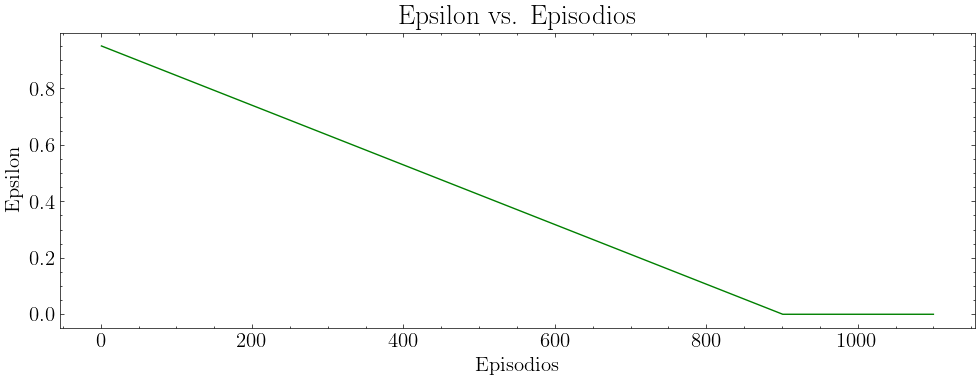
\includegraphics[scale=0.6]{figs/Diseño/RL/epsilon.png}
  \end{center}
  \caption{Gráfica del valor de epsilon respecto al episodio}
  \label{fig:epsilon}
  \vspace{-1.5em}
\end{figure}
  \end{itemize}

  El algoritmo Q-learning se basa en seguir una función acción-recompensa formada por un tabla estado-acción la cual se va rellenando siguiendo la ecuación
  de Bellman\cite{Bellman} mostrada en la ecuación \ref{eq:bellman}.
  \begin{myequation}[ht]
    \begin{equation}
      Q(s, a) = Q(s, a) + \alpha \cdot [R(s, a) + \gamma \cdot \max Q(s', a') - Q(s, a)]
      \label{eq:bellman}
    \end{equation}
    \caption{Ecuación de Bellman}
  \end{myequation}
  en donde, 
  \begin{itemize}
    \item \textbf{$Q(s, a)$}: Valor Q para el estado $s$ y la acción $a$. Se trata de una matriz formada por estado y acción que se rellena durante la fase de entrenamiento para utilizarla
    en la fase de inferencia.
    \item \textbf{$\alpha$}: Tasa de aprendizaje entre un valor de 0 a 1. Consiste en el porcentaje que daremos al agente para el proceso de aprendizaje, 
    si dicho valor es alto daremos más peso al valor aprendido. Dicho valor se define con un valor de 0.5 
    \item \textbf{$R(s, a)$ }: Recompensa por tomar la acción $a$ en el estado $s$. La función de recompensa es crucial en el proceso de aprendizaje del agente, 
    evalúa como es de buena la acción tomada por el agente en el estado que se encuentre. Proporciona información al agente sobre que acciones maximizan la recompensa total a lo largo del tiempo. Dicha función
    de recompensa es diseñada dependiendo de cual sea el objetivo de tu agente. 
    \item \textbf{$\gamma$}: Factor de descuento entre un valor de 0 a 1. Modela la importancia de las recompensas futuras en relación con las recompensas inmediatas, refleja la importancia del agente
    por las recompensas a largo plazo. Un valor alto significará que le agente valorará mucho las recompensas futuras, mientras que un valor bajo indica que se enfocará más en las recompensas
    inmediatas. Dicho valor se define con un valor de 0.7.
    \item \textbf{$\max Q(s', a')$}: Valor Q máximo en el próximo estado $s'$ para todas las acciones posibles $a'$.
\end{itemize}

\subsubsection{Fase de entrenamiento}
\label{sec:entrenamiento}
 Dentro de esta fase, existen dos conceptos importantes a destacar:
 \begin{itemize}
  \item \textbf{Episodios}: Se define episodio como una secuencia completa de interacciones que se produce entre el agente y el entorno. Cada episodio comienza con un estado inicial y consta de una serie 
  de pasos o acciones tomadas por el agente.
  \item \textbf{Iteraciones}: Son los pasos que puede dar un agente en el entorno dentro de un episodio. Estos pasos pueden incluir observaciones del entorno, decisiones tomadas por el agente
  y las consecuentes recompensas o penalizaciones recibidas.
\end{itemize}

 La fase de entrenamiento consiste que el agente explore todo lo máximo posible en el entorno respecto a los estados que tiene y las acciones que puede tomar, es decir, al comienzo del 
 entrenamiento se inicializa la tabla Q(S,A) a cero todos sus valores y mediante el algoritmo de Q-learning, se va rellenando hasta converger el modelo.
 
 Básicamente, en cada iteración del algoritmo, se escoge una acción según si el agente se encuentra en exploración o explotación, se calcula la recompensa obtenida y se actualiza la 
 tabla de nuevo sobre el algoritmo.

 El entrenamiento finaliza cuando el agente haya aprendido, es decir, el agente ha cumplido el objetivo. Esto sucede cuando las iteraciones del algoritmo y la recompensa acumulada del agente en esta 
 fase se estabilicen y tengan valores constantes, es decir, no cambian significativamente con más iteraciones. Esto significa que el modelo ha convergido y a continuación se pasa
 a la fase de inferencia. 

Durante la fase de entrenamiento, el algoritmo se ejecuta continuamente. Como se menciona en la sección \ref{sec:Análisis del algoritmo de percepción}, el sistema de percepción tiene 30 frames por
segundo, proporcionando al agente información visual del entorno en tiempo real. Sin embargo, para permitir al agente tomar decisiones más efectivas y gestionar adecuadamente las acciones 
y estados del entorno, se reduce el tiempo global de procesamiento del algoritmo a 10 frames por segundo. Esto asegura que el agente tenga suficiente tiempo para analizar cada acción y estado. La ejecución de este 
algoritmo de entrenamiento es aproximadamente de 12 horas, asegurando que el algoritmo va ser capaz de completar el entrenamiento de manera correcta consiguiendo converger. 

En la figura \ref{fig:iteraciones} 
se muestra la evolución de las iteraciones que tiene el dron con el entorno en función del episodio. Al comienzo del entrenamiento, el dron obtiene bajas iteraciones, esto se debe a que 
al comienzo del entrenamiento desconoce completamente el entorno y las acciones que debe realizar. Pero, no obstante, a medida que el entrenamiento va avanzando, 
las iteraciones obtienen valores altos hasta llegar al episodio
900 donde la fase de exploración finaliza y comienza la fase de explotación siendo epsilon 0 como se muestra en la figura \ref{fig:epsilon}. A partir de este punto, las iteraciones tienen 
una tendencia ascendente con pequeñas variaciones, estas variaciones se deben a que en la fase de entrenamiento el dron no comienza siempre en el mismo punto de inicio como 
se muestra en la figura \ref{fig:Entorno}, obteniendo en cada punto de partida hasta el final del recorrido una serie de iteraciones. Aunque se muestren estas pequeñas variaciones, el modelo
ha sido capaz de converger debido a que el dron es capaz de completar el recorrido continuamente sin salirse del carril.

\begin{figure} [H]
  \begin{center}
    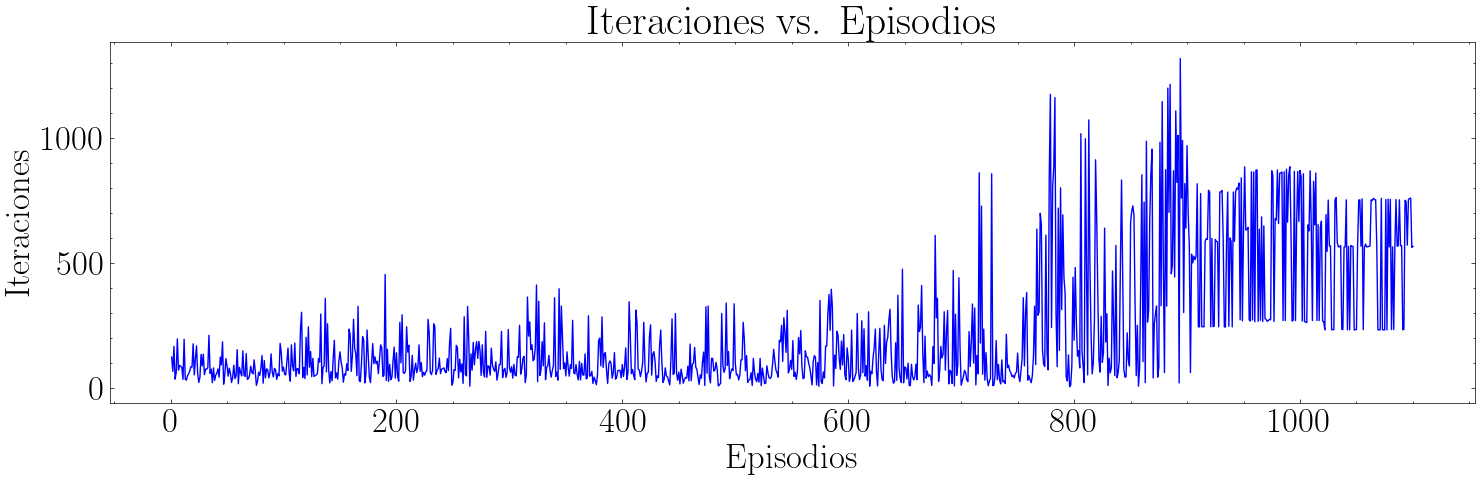
\includegraphics[scale=0.4]{figs/Diseño/RL/steps.png}
  \end{center}
  \caption{Gráfica de las iteraciones respecto al episodio}
  \label{fig:iteraciones}
  \vspace{-1.5em}
\end{figure}

Respecto a la evolución de la función de recompensa, se puede observar en la figura \ref{fig:recompensa} como la recompensa acumulativa va obteniendo valores ascendentes a medida que el dron 
aprende del entorno para no salirse del carril. En el momento en que se llega al episodio 900, la recompensa acumulativa tiende a ser siempre ascendente teniendo pequeñas variaciones entre los 
episodios. Este comportamiento ocurre como las iteraciones, se producen pequeñas variaciones debido a los puntos de partida que tiene el dron durante cada comienzo de su entrenamiento. A partir 
del momento 
que no se produzca grandes variaciones respecto a las iteraciones y la recompensa acumulativa en función de los episodios, se puede decir que el modelo ha sido capaz de converger. Esto significa
que el dron completa satisfactoriamente el recorrido en cualquier punto de partida definido. Una vez analizado los resultados del entrenamiento con las diferentes métricas, se da a pie a la 
fase de inferencia para verificar el resultado obtenido con el modelo convergido.

\begin{figure} [H]
  \begin{center}
    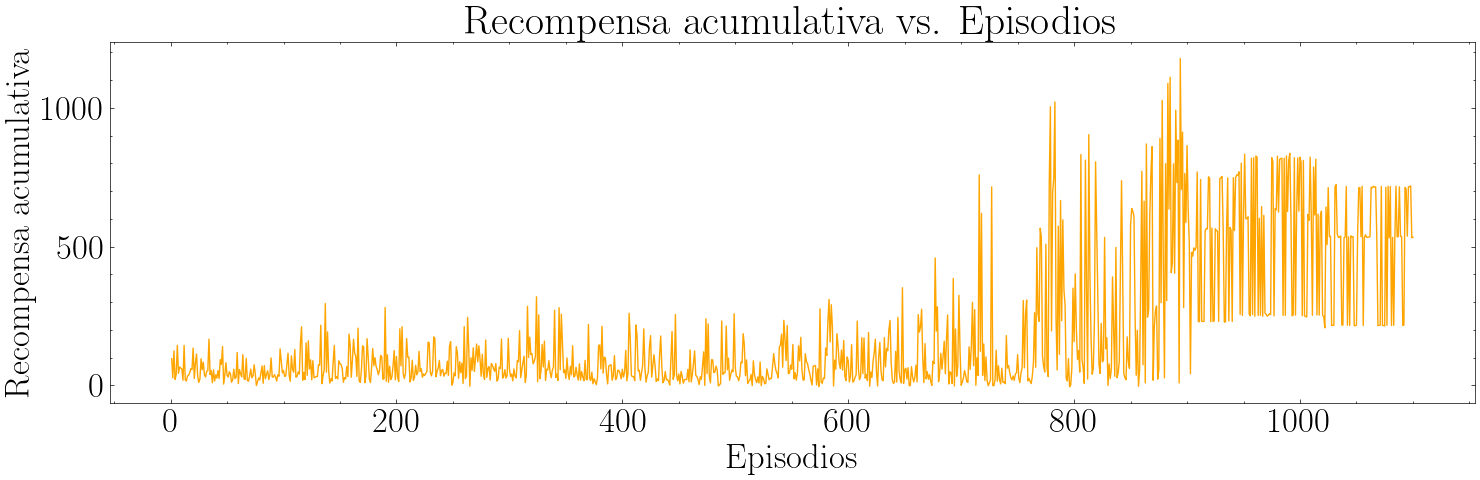
\includegraphics[scale=0.4]{figs/Diseño/RL/recompensa.png}
  \end{center}
  \caption{Gráfica de la recompensa acumulativa en función de los episodios}
  \label{fig:recompensa}
  \vspace{-1.5em}
\end{figure}

\subsubsection{Fase de inferencia}
\label{sec:fases_inferencia}
La fase de inferencia consiste en indexar la tabla Q(S,A) que se ha ido rellenando en la fase de entrenamiento. El dron cuando se encuentre en un estado especifico consultará la tabla Q(S,A) para
encontrar la mejor acción en ese estado (cuando mencionamos la mejor acción nos referimos al máximo valor en la tabla que tenga en ese estado). Cuando el dron tome dicha acción se moverá al siguiente estado
siendo así un proceso iterativo hasta alcanzar la meta. En esta fase, los valores de la tabla permanecen constantes y se utiliza para la toma de decisiones basadas en el conocimiento
aprendido en la fase de entrenamiento.

En la figura \ref{fig:Distribucción_inferencia} se puede observar las diferentes acciones que ha utilizado el dron para completar el recorrido utilizando cuatro de las veintiuno acciones
disponibles. Aunque se muestre solamente cuatro acciones utilizadas, durante la fase de entrenamiento, el dron ha aprendido muchas más acciones y estados como se muestran. 

Se destaca que la acción más usada se trata de una de las acciones que presentan poco giro y alta velocidad lineal dentro de las acciones con más velocidad lineal, esto se debe
a la importancia de la función de recompensa al considerar que queremos que el dron se mantenga constantemente en el centro del carril manteniendo un ángulo de orientación adecuado
sin salirse del carril. En la figura \ref{fig:inferencia-imagenes}, se muestra una serie de imágenes durante la inferencia del modelo en el recorrido donde el dron ha sido entrenado, manteniendo una trayectoria 
estable respecto al centro del carril.

\begin{figure} [H]
  \begin{center}
    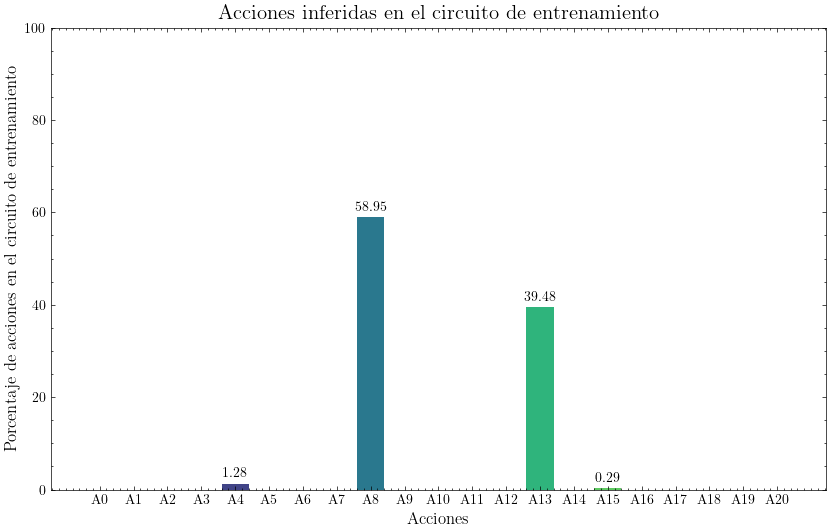
\includegraphics[scale=0.3]{figs/Diseño/RL/Acciones_inferidas.png}
  \end{center}
  \caption{Distribución de acciones en inferencia}
  \label{fig:Distribucción_inferencia}
\end{figure}

\begin{figure}[H]
  \centering
  \begin{minipage}{0.3\textwidth}
    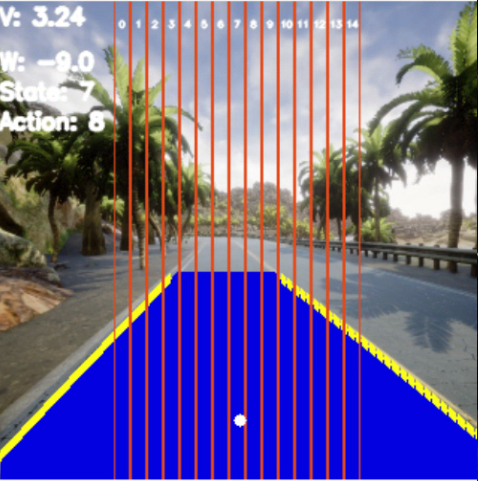
\includegraphics[width=\linewidth]{figs/Diseño/RL/RL1.png}
  \end{minipage}
  \hfill
  \begin{minipage}{0.3\textwidth}
    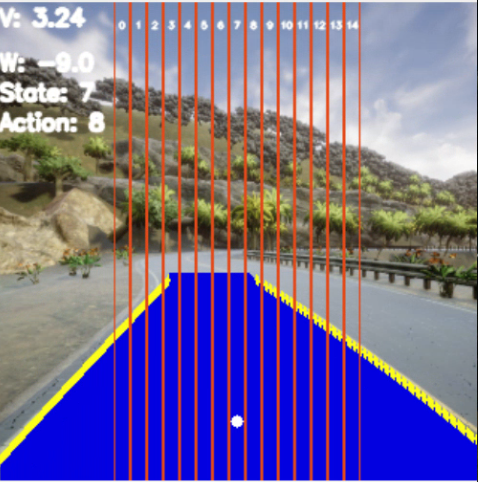
\includegraphics[width=\linewidth]{figs/Diseño/RL/RL3.png}
  \end{minipage}
  \hfill
  \begin{minipage}{0.3\textwidth}
    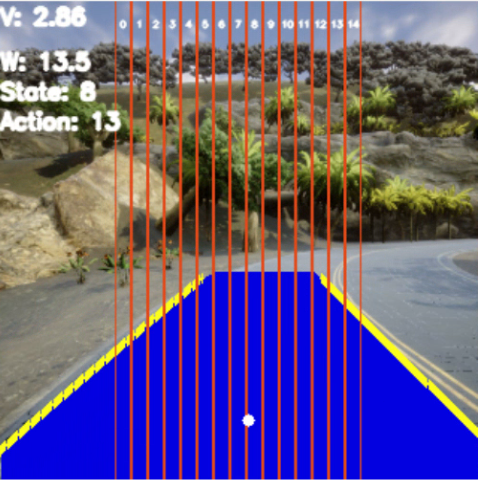
\includegraphics[width=\linewidth]{figs/Diseño/RL/RL4.png}
  \end{minipage}
  \hfill
  \begin{minipage}{0.3\textwidth}
    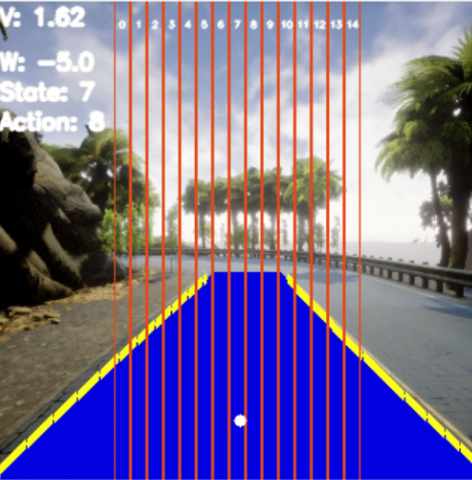
\includegraphics[width=\linewidth]{figs/Diseño/RL/RL5.png}
  \end{minipage}
  \caption{Resultado del comportamiento de aprendizaje por refuerzo ilustrando los estados y acciones en la fase de inferencia}
  \label{fig:inferencia-imagenes}
  \vspace{-1.5em}
\end{figure}

Como resultado al utilizar el algoritmo de Q-learning, el modelo entrenado ofrece tener un resultado eficaz a la hora de navegar por el entorno, pudiendo observar 
el modelo entrenado final en diferentes localizaciones aleatorias en el entorno como se muestra en la figura \ref{fig:Entorno}. 
Aunque el algoritmo obtiene un rate de 10 FPS como se menciona en la sección \ref{sec:entrenamiento}, se han explorado los límites de velocidad angular y lineal que el dron puede alcanzar mientras navega. Se multiplica tanto la velocidad angular como la lineal
por un factor. La velocidad lineal es multiplicado por 2.0 y la velocidad angular por 1.8 consiguiendo aumentar un 100\% las acciones. Este proceso es interesante realizarlo para 
maximizar el modelo entrenado sin necesidad de volver a entrenar un nuevo modelo, demostrando que el modelo es efectivo al aumentar el valor de las acciones.

Los nuevos
valores de las acciones originales como se muestran en la figura \ref{fig:Acciones} son multiplicados por ambos factores
y su gráfico de acciones como se muestra en la figura \ref{fig:inferencia_factor}. Se puede observar que en la distribución de acciones el dron
sigue escogiendo acciones con velocidad lineal alta y velocidad angular baja para mantenerse dentro del recorrido sin salirse, además de aumentar el porcentaje de las acciones escogidas respecto a la distribución de acciones
que se muestra en la figura \ref{fig:Distribucción_inferencia}

\begin{figure} [H]
  \begin{center}
    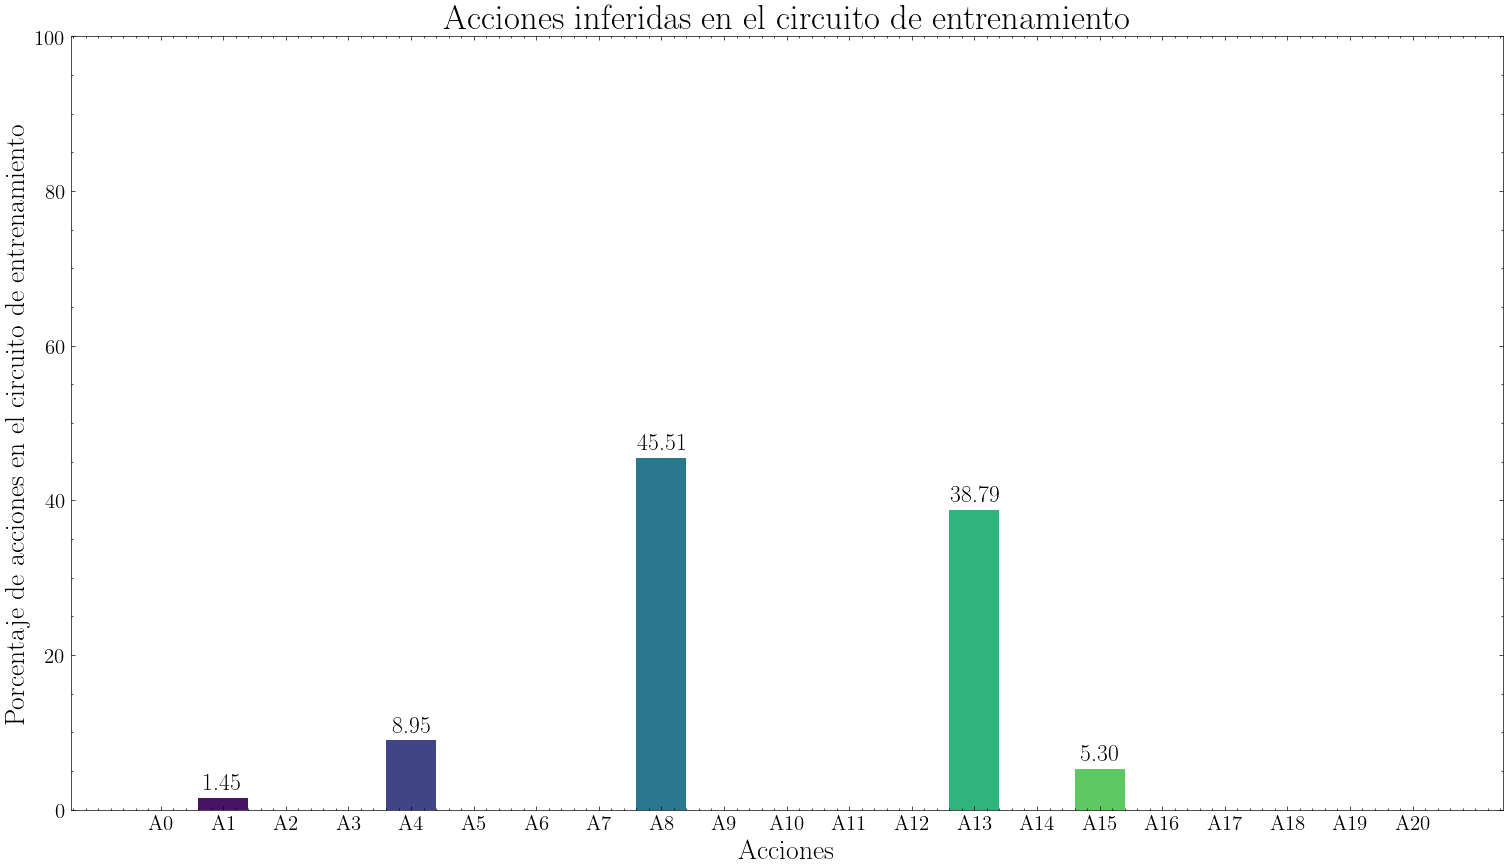
\includegraphics[scale=0.3]{figs/Diseño/RL/Acciones_inferidas_factor.png}
  \end{center}
  \caption{Distribución de acciones en inferencia}
  \label{fig:inferencia_factor}
\end{figure}

\subsection{Comparativa PID vs Q-learning}
\label{sec:Análisis y comparativa entre el seguiento de carril clásico}
Para comprobar la robustez y la eficacia que demuestra el modelo entrenado con aprendizaje por refuerzo respecto al seguimiento de carril mediante el PID, se realiza varias comparativas, en ambos
comportamientos se utiliza el mismo sistema perceptivo que se menciona en la sección \ref{sec:Percepción}. 

Se definen límites a las velocidades (lineales y angulares) del controlador PID para que ambos tengan las mismas condiciones, siendo que el controlador PID tenga los mismos 
rangos mínimos y máximos de velocidades como Q-learning. Para realizar la comparativa, se ha escogido un escenario en el que ambos comportamientos visitan por primera vez 
sin que ninguno de los dos comportamientos se salgan del carril. En la figura \ref{fig:escenario-comparativa} se muestra el escenario marcando el inicio 
y el final del recorrido, además de la vista que tiene el dron al comienzo del recorrido.


\begin{figure} [H]
  \begin{center}
    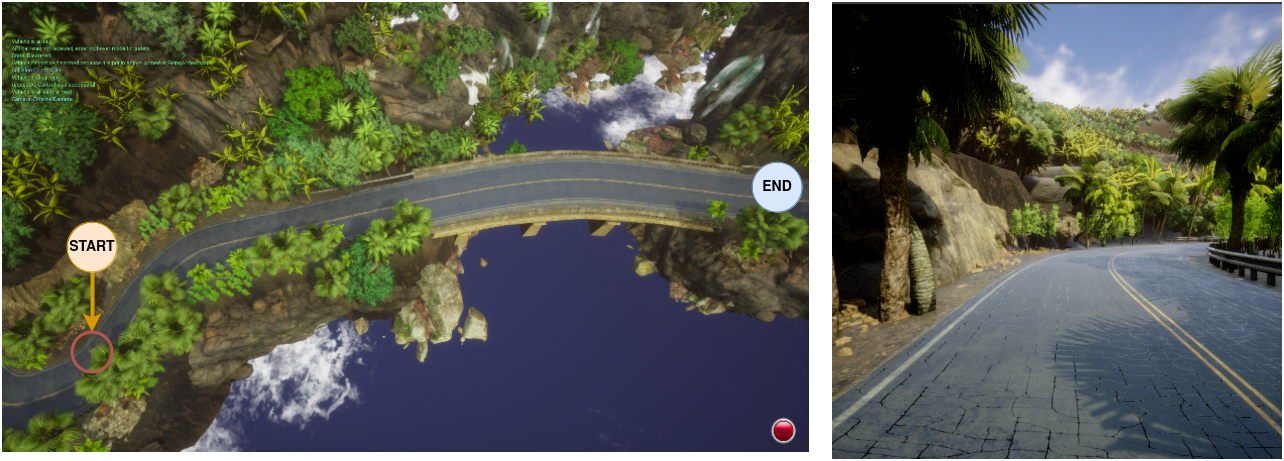
\includegraphics[scale=0.33]{figs/Diseño/RLvsPID/escenario.png}
  \end{center}
  \caption{Escenario de control tradicional y aprendizaje por refuerzo}
  \label{fig:escenario-comparativa}
\end{figure}

Para realizar como ha sido la trayectoria de ambos comportamientos dentro del escenario, se ha ido recogiendo en cada momento la posición del dron (x,y) durante su navegación
 para más adelante contrastarlos. En la figura \ref{fig:Comparativa-de-trayectorias}, se muestra una comparativa de trayectorias entre PID y Q-learning 
realizando un zoom en una de las partes de ambas 
trayectorias.

\begin{figure}[H]
  \centering
  \begin{minipage}{0.65\textwidth}
    \includegraphics[width=\linewidth]{figs/Diseño/RLvsPID/zona-trayecto-zoom.png}
  \end{minipage}

  \vspace{1cm}

  \begin{minipage}{0.65\textwidth}
    \includegraphics[width=\linewidth]{figs/Diseño/RLvsPID/zona-trayecto.png}
  \end{minipage}
  \caption{Comparativa de trayectorias entre el control clásico y el control de aprendizaje por refuerzo}
  \label{fig:Comparativa-de-trayectorias}
  \vspace{-1.5em}
\end{figure}

Como se observa en esta comparativa, una de las principales diferencias entre ambos comportamientos es que el control clásico basado en el PID presenta oscilaciones durante el recorrido 
realizando eses consiguiendo una velocidad angular media alrededor de 0.9 grados/segundos hasta llegar al punto final.  

En cambio, el comportamiento con aprendizaje por refuerzo destaca por su trayectoria constante durante todo el recorrido sin apenas realizar oscilaciones obteniendo una velocidad angular 
media de 0.1 grados/segundos siendo menor que el resultado del controlador PID. Esto se debe a que el controlador PID constantemente tiene que estar realizando ajustes de velocidades 
angulares para mantenerse centrado y dentro del carril, sin embargo con comportamiento de aprendizaje por refuerzo es capaz de aprender y adaptarse con una velocidad angular baja 
realizando giros menos bruscos. 

\begin{figure}[H]
  \centering
  \begin{minipage}{0.3\textwidth}
    \includegraphics[width=\linewidth]{figs/Diseño/RLvsPID/RL1.png}
  \end{minipage}
  \hfill
  \begin{minipage}{0.3\textwidth}
    \includegraphics[width=\linewidth]{figs/Diseño/RLvsPID/RL2.png}
  \end{minipage}
  \hfill
  \begin{minipage}{0.3\textwidth}
    \includegraphics[width=\linewidth]{figs/Diseño/RLvsPID/RL3.png}
  \end{minipage}
  \hfill
  \begin{minipage}{0.3\textwidth}
    \includegraphics[width=\linewidth]{figs/Diseño/RLvsPID/RL4.png}
  \end{minipage}
  \caption{Resultado del comportamiento de aprendizaje por refuerzo}
  \label{fig:Resultado-imagenes}
  \vspace{-1.5em}
\end{figure}

Demostrando así que el modelo entrenado es capaz de obtener comportamientos satisfactorios tomando acciones acordes a diferentes escenarios. En la figura \ref{fig:Resultado-imagenes}, 
se muestra una secuencia de frames
del comportamiento de aprendizaje por refuerzo durante el recorrido siendo capaz de mantenerse centrado al carril, mostrando las acciones y en que estado se encuentra.

En este otro experimento, se realiza un análisis entre el PID y Q-learning, en el cual ambos comportamientos tienen los mismos rangos de velocidades mínimas y máximas y demostrando que
el controlador PID no es capaz de mantenerse dentro del carril desembocando que se salga 
del carril. Se utiliza un escenario en el que ambos comportamientos visitan por primera vez, este escenario se puede visualizar en la figura \ref{fig:escenario-comparativa-II} junto 
con la vista del dron. Se trata de un escenario en donde presenta curvas hacia la derecha e izquierda.

\begin{figure} [H]
  \begin{center}
    \includegraphics[scale=0.34]{figs/Diseño/RLvsPID/comparativa-II.png}
  \end{center}
  \caption{Escenario II de control tradicional y aprendizaje por refuerzo}
  \label{fig:escenario-comparativa-II}
  \vspace{-1.5em}
\end{figure}

En este análisis, se evalúa trayectoria que han seguido ambos comportamientos como se muestra en la figura \ref{fig:Trayecto-II}. 

\begin{figure} [H]
  \begin{center}
    \includegraphics[scale=0.35]{figs/Diseño/RLvsPID/sale-pid/trayecto.png}
  \end{center}
  \caption{Trayecto del comportamiento PID y Q-learning}
  \label{fig:Trayecto-II}
  \vspace{-1.5em}
\end{figure}

Al comienzo del recorrido, tanto el controlador PID como Q-learning
son capaces de mantener una trayectoria suave y centrada respecto al centro del carril. Esto indica que ambos métodos pueden manejar bien las condiciones iniciales del entorno. En cambio, cuando 
el dron se enfrenta a la primera curva, comienza a surgir diferencias notables. El controlador PID empieza a oscilar, tratando de corregir su posición para mantenerse dentro del carril. Estas 
oscilaciones son típicas de un sistema PID tratando de adaptarse rápidamente a cambios en la trayectoria. En contraste, el algoritmo Q-learning mantiene una trayectoria acorde a la curva 
sin realizar ninguna oscilación significativa, mostrando una mayor estabilidad. Debido a las oscilaciones del PID, el dron llega a un punto donde no puede mantenerse dentro del carril, saliéndose 
de la trayectoria. Esto se destaca en la gráfica, donde se marca la \textbf{"Salida del carril PID"}. Por otro lado, el comportamiento de Q-learning sigue la trayectoria  de forma consistente 
y centrada, completando el recorrido sin salirse del carril.

Esta comparativa de las trayectorias revela que el algoritmo de Q-learning ofrece mejores resultados en cuanto al controlador PID. Mientras que el PID sufre oscilaciones y se sale de la trayectoria,
Q-learning demuestra una capacidad para adaptarse al recorrido, completándolo de manera eficiente y manteniéndose dentro del carril.



En la figura \ref{comparativa-PID-qlearning} se muestran varios frames de ambos comportamientos durante la trayectoria mostrando como Q-learning mantiene una trayectoria robusta y centrada 
en comparación con el PID. En particular, en la tercera columna se observa cómo el controlador PID se desvía su trayectoria, mientras que Q-learning sigue su trayecto con éxito. 
Estos resultados subrayan la importancia de utilizar métodos de control adaptativos que tienen la capacidad de generalizar y ser flexibles
como Q-learning para aplicaciones de navegación autónomas con drones en carreteras, donde los métodos 
tradicionales pueden no ser suficientes para garantizar un rendimiento fiable. 

\begin{figure}[H]
  \centering

  % Título para la primera fila
  \textbf{PID}
  \vspace{0.3cm}

  \begin{minipage}[t]{0.2\textwidth}
      \centering
      \includegraphics[width=\textwidth]{figs/Diseño/RLvsPID/sale-pid/PID1.png}
      \caption*{}
  \end{minipage}
  \hfill
  \begin{minipage}[t]{0.2\textwidth}
      \centering
      \includegraphics[width=\textwidth]{figs/Diseño/RLvsPID/sale-pid/PID2.png}
      \caption*{}
  \end{minipage}
  \hfill
  \begin{minipage}[t]{0.2\textwidth}
      \centering
      \includegraphics[width=\textwidth]{figs/Diseño/RLvsPID/sale-pid/PID3.png}
      \caption*{}
  \end{minipage}
  \hfill
  \begin{minipage}[t]{0.2\textwidth}
      \centering
      \includegraphics[width=\textwidth]{figs/Diseño/RLvsPID/sale-pid/PID4.png}
      \caption*{}
  \end{minipage}
  \vspace{0.5cm}

  % Título para la segunda fila
  \textbf{Q-learning}
  \vspace{0.3cm}

  \begin{minipage}[t]{0.2\textwidth}
      \centering
      \includegraphics[width=\textwidth]{figs/Diseño/RLvsPID/sale-pid/RL1.png}
  \end{minipage}
  \hfill
  \begin{minipage}[t]{0.2\textwidth}
      \centering
      \includegraphics[width=\textwidth]{figs/Diseño/RLvsPID/sale-pid/RL2.png}
  \end{minipage}
  \hfill
  \begin{minipage}[t]{0.2\textwidth}
      \centering
      \includegraphics[width=\textwidth]{figs/Diseño/RLvsPID/sale-pid/RL3.png}
  \end{minipage}
  \hfill
  \begin{minipage}[t]{0.2\textwidth}
      \centering
      \includegraphics[width=\textwidth]{figs/Diseño/RLvsPID/sale-pid/RL4.png}
  \end{minipage}
  % Caption general para la figura
  \caption{Comparativa entre el PID y Q-learning}
  \label{comparativa-PID-qlearning}
\end{figure}


  

